\documentclass[11pt, twoside, openright]{memoir}

% ── Core packages ─────────────────────────────────────────────────────────────
\usepackage{amsmath, amssymb, bm}
\usepackage{mathtools}
\usepackage[T1]{fontenc}
\usepackage[utf8]{inputenc}
\usepackage{palatino}
\usepackage{mathpazo}
\usepackage{microtype}

% ── Page geometry ─────────────────────────────────────────────────────────────
\usepackage[
  letterpaper,
  top=1in, bottom=1in,
  inner=1in, outer=1in,
  includeheadfoot
]{geometry}

% ── Graphics, tables, color ───────────────────────────────────────────────────
\usepackage{graphicx}
\usepackage{booktabs}
\usepackage{array}
\usepackage{tabularx}
\usepackage[table]{xcolor}
\usepackage[most]{tcolorbox}
\usepackage{tikz}
\usetikzlibrary{arrows.meta, calc, positioning, decorations.pathreplacing}
\usepackage{listings}

% ── Lists, floats ─────────────────────────────────────────────────────────────
\usepackage{enumitem}
\usepackage{parskip}
\usepackage{float}
\usepackage{caption}
\captionsetup{font=small, labelfont=bf}

% ── References ────────────────────────────────────────────────────────────────
\usepackage{hyperref}
\hypersetup{colorlinks=true, linkcolor=Navy, urlcolor=Blue, citecolor=Teal,
  pdftitle={Learning Geometric Algebra Through Transformer Geometry},
  pdfauthor={Agus Sudjianto, Sandi Setiawan, and Aijun Zhang}}

% ── Colors ────────────────────────────────────────────────────────────────────
\definecolor{Navy}{HTML}{1F3864}
\definecolor{Blue}{HTML}{2E6DAD}
\definecolor{LBlue}{HTML}{DDEAF7}
\definecolor{Teal}{HTML}{1D6A6A}
\definecolor{LTeal}{HTML}{D6EFEF}
\definecolor{Amber}{HTML}{7B4A00}
\definecolor{LAmber}{HTML}{FFF3CD}
\definecolor{DGreen}{HTML}{1B5E20}
\definecolor{LGreen}{HTML}{E8F5E9}
\definecolor{DRed}{HTML}{7B1515}
\definecolor{LRed}{HTML}{FDECEA}
\definecolor{LGray}{HTML}{F5F5F5}
\definecolor{MGray}{HTML}{DDDDDD}
\definecolor{DGray}{HTML}{444444}
\definecolor{CodeBG}{HTML}{F7F7F7}
\definecolor{Purple}{HTML}{5B2C8B}
\definecolor{LPurple}{HTML}{EDE7F6}

% ── Memoir styles ─────────────────────────────────────────────────────────────
\chapterstyle{veelo}
\renewcommand{\partnamefont}{\huge\sffamily\color{Navy}}
\renewcommand{\partnumfont}{\huge\sffamily\color{Navy}}
\renewcommand{\parttitlefont}{\Huge\bfseries\sffamily\color{Navy}}
\setsecheadstyle{\large\bfseries\sffamily\color{Navy}}
\setsubsecheadstyle{\normalsize\bfseries\sffamily\color{Blue}}
\setsubsubsecheadstyle{\normalsize\bfseries\itshape\color{Teal}}
\pagestyle{ruled}

% ── tcolorbox environments ─────────────────────────────────────────────────────
\tcbset{
  base/.style={enhanced, breakable, left=6pt, right=6pt, top=6pt, bottom=6pt,
    fontupper=\small, before upper={\parskip=4pt}, arc=3pt, boxrule=1pt},
}
\newtcolorbox{whycare}{base, colback=LAmber, colframe=Amber,
  title={\sffamily\bfseries\small\color{white}~Why This Matters},
  attach boxed title to top left={yshift=-2mm, xshift=6mm},
  boxed title style={colback=Amber, arc=2pt, boxrule=0pt}}
\newtcolorbox{keyidea}{base, colback=LGreen, colframe=DGreen,
  title={\sffamily\bfseries\small\color{white}~Key Idea},
  attach boxed title to top left={yshift=-2mm, xshift=6mm},
  boxed title style={colback=DGreen, arc=2pt, boxrule=0pt}}
\newtcolorbox{analogy}{base, colback=LBlue, colframe=Blue,
  title={\sffamily\bfseries\small\color{white}~Analogy},
  attach boxed title to top left={yshift=-2mm, xshift=6mm},
  boxed title style={colback=Blue, arc=2pt, boxrule=0pt}}
\newtcolorbox{tryit}{base, colback=LTeal, colframe=Teal,
  title={\sffamily\bfseries\small\color{white}~Try It Yourself},
  attach boxed title to top left={yshift=-2mm, xshift=6mm},
  boxed title style={colback=Teal, arc=2pt, boxrule=0pt}}
\newtcolorbox{pitfall}{base, colback=LRed, colframe=DRed,
  title={\sffamily\bfseries\small\color{white}~Common Pitfall},
  attach boxed title to top left={yshift=-2mm, xshift=6mm},
  boxed title style={colback=DRed, arc=2pt, boxrule=0pt}}
\newtcolorbox{finding}{base, colback=LGreen, colframe=DGreen,
  title={\sffamily\bfseries\small\color{white}~What the Data Shows},
  attach boxed title to top left={yshift=-2mm, xshift=6mm},
  boxed title style={colback=DGreen, arc=2pt, boxrule=0pt}}
\newtcolorbox{mathbox}{base, colback=LGray, colframe=MGray,
  title={\sffamily\bfseries\small\color{DGray}~Under the Hood},
  attach boxed title to top left={yshift=-2mm, xshift=6mm},
  boxed title style={colback=MGray, arc=2pt, boxrule=0pt}}
\newtcolorbox{gabox}{base, colback=LPurple, colframe=Purple,
  title={\sffamily\bfseries\small\color{white}~GA Concept},
  attach boxed title to top left={yshift=-2mm, xshift=6mm},
  boxed title style={colback=Purple, arc=2pt, boxrule=0pt}}
\newtcolorbox{transformer}{base, colback=LBlue, colframe=Navy,
  title={\sffamily\bfseries\small\color{white}~In the Transformer},
  attach boxed title to top left={yshift=-2mm, xshift=6mm},
  boxed title style={colback=Navy, arc=2pt, boxrule=0pt}}

% ── Code listings ─────────────────────────────────────────────────────────────
\lstset{
  language=Python,
  basicstyle=\ttfamily\footnotesize,
  backgroundcolor=\color{CodeBG},
  frame=single,
  rulecolor=\color{MGray},
  keywordstyle=\color{Blue}\bfseries,
  commentstyle=\color{DGreen}\itshape,
  stringstyle=\color{DRed},
  numbers=left,
  numberstyle=\tiny\color{MGray},
  numbersep=5pt,
  breaklines=true,
  showstringspaces=false,
  tabsize=4,
  xleftmargin=10pt,
  xrightmargin=5pt,
  aboveskip=8pt,
  belowskip=8pt,
}

% ── Table column types ────────────────────────────────────────────────────────
\newcolumntype{L}[1]{>{\raggedright\arraybackslash}p{#1}}
\newcolumntype{C}[1]{>{\centering\arraybackslash}p{#1}}

% ── GA math commands ──────────────────────────────────────────────────────────
\newcommand{\gp}{\,}              % geometric product (juxtaposition)
\newcommand{\ip}{\cdot}           % inner product
\newcommand{\op}{\wedge}          % outer (wedge) product
\newcommand{\rev}[1]{\widetilde{#1}} % reversion
\newcommand{\grade}[2]{\langle #1 \rangle_{#2}} % grade projection
\newcommand{\rotor}[1]{\mathcal{R}^{(#1)}}  % rotor at layer l
\newcommand{\bivec}[1]{\mathcal{B}^{(#1)}}  % bivector at layer l
\newcommand{\metric}[1]{\mathcal{P}^{(#1)}} % metric factor at layer l

% ── Misc ──────────────────────────────────────────────────────────────────────
\setlength{\parindent}{0pt}
\setlength{\parskip}{6pt}

% ══════════════════════════════════════════════════════════════════════════════
\begin{document}
% ══════════════════════════════════════════════════════════════════════════════

\frontmatter
\pagestyle{empty}


% ── Title page ────────────────────────────────────────────────────────────────
\begin{titlingpage}
\vspace*{1.5cm}
\begin{center}
  {\color{Navy}\rule{\linewidth}{2pt}}\\[12pt]
  {\Huge\bfseries\sffamily\color{Navy} Learning Geometric Algebra}\\[10pt]
  {\LARGE\bfseries\sffamily\color{Navy} Through Transformer Geometry}\\[10pt]
  {\color{Navy}\rule{\linewidth}{1.5pt}}\\[20pt]
  {\large\sffamily\color{DGray} Agus Sudjianto}\\[16pt]
  {\large\sffamily\color{DGray} Sandi Setiawan}\\[16pt]
  {\large\sffamily\color{DGray} Aijun Zhang}\\[40pt]
  {\normalsize\itshape\color{DGray}
   A self-guided introduction to Geometric Algebra\\
   with language models as your laboratory}\\[30pt]
  {\small\sffamily\color{DGray} Version: March 25, 2026}\\[20pt]
  {\small\sffamily\color{Blue}
   \href{https://github.com/asudjianto-xml/GA-Transformer-Geometry}%
   {github.com/asudjianto-xml/GA-Transformer-Geometry}}
\end{center}
\end{titlingpage}
\clearpage

% ── Preface ───────────────────────────────────────────────────────────────────
\chapter*{Preface}
\addcontentsline{toc}{chapter}{Preface}

\subsection*{What this book is}

This is a book about Geometric Algebra.  It teaches you a powerful
mathematical framework --- the Clifford algebra $\mathrm{Cl}(k, 0)$ ---
through a concrete, fascinating application: understanding how large
language models process information internally.

You will learn GA one concept at a time.  Each chapter introduces a single
algebraic idea, develops it with small examples you can work by hand, and
then immediately applies it to real data extracted from a transformer
language model.  The transformer is your \emph{laboratory}: a place where
abstract algebraic concepts become visible, measurable, and surprising.

\subsection*{Why transformers?}

Geometric Algebra was born in physics and has thrived in computer graphics,
robotics, and signal processing.  But transformers offer something these
fields do not: a high-dimensional space ($k = 256$ after whitening) where
\emph{every} GA concept --- bivectors, rotors, holonomy, commutators ---
appears naturally in the data.  In 3D physics, a bivector is just a
dressed-up cross product.  In $\mathbb{R}^{256}$, bivectors have
$32{,}640$ independent components, multiple principal planes, and rich
internal structure.  This is where GA earns its keep.

Moreover, transformers are \emph{important}.  Understanding their internal
computation is one of the central challenges in AI.  By learning GA
through this lens, you gain two things at once: a deep understanding of
a beautiful algebra, and a new way to see inside the models that are
reshaping technology.

\subsection*{What you need}

\begin{itemize}[nosep]
\item \textbf{Linear algebra}: matrix multiplication, eigenvalues,
  orthogonal matrices, SVD.  A first undergraduate course is sufficient.
\item \textbf{Python}: NumPy-level comfort.  The code is simple and
  self-contained.
\item \textbf{Calculus}: partial derivatives for the dependency chapter.
  You can skip that chapter if needed.
\item \textbf{No prior GA knowledge.}  We start from vectors.
\item \textbf{No prior ML knowledge.}  Appendix~\ref{app:transformers}
  covers everything you need about transformers.
\end{itemize}

\subsection*{How to read this book}

Each chapter follows the same pattern:

\begin{enumerate}[nosep]
\item \textbf{The GA concept} --- introduced abstractly with small
  ($\mathbb{R}^3$ or $\mathbb{R}^4$) examples.
\item \textbf{In the transformer} --- the same concept applied to real
  hidden-state data from a language model.
\item \textbf{Code} --- working Python using the \texttt{layer\_time\_ga}
  library.  Every code block runs in the companion Jupyter notebooks.
\item \textbf{Exercises} --- both pure GA problems and transformer-data
  explorations.
\end{enumerate}

The chapters build sequentially: each depends on the previous.  Read them
in order the first time.  After that, use the chapters as reference.

\subsection*{Three kinds of statement}

This book mixes mathematics, computation, and empirical observation.  To
keep the distinction clear, we use three categories throughout:

\begin{itemize}[nosep]
\item \textbf{GA identity} (exact).  A mathematical fact that holds in any
  Clifford algebra $\mathrm{Cl}(k, 0)$.  Example: the geometric product
  decomposes as $ab = a \ip b + a \op b$.  These do not depend on any
  model or dataset.
\item \textbf{Computational construction} (defined).  A procedure we
  define and apply to transformer data: whitening, the layer transition
  operator, versor decomposition, dependency density, etc.  These are
  methodological choices, not theorems.
\item \textbf{Empirical observation} (observed).  A pattern we find in
  a specific model under a specific setup --- for instance, that grade-0
  dominates grade-2 in late layers of Qwen2.5-7B.  These observations
  motivate the narrative, but they are not guaranteed to hold for all
  models, prompts, or whitening dimensions.
\end{itemize}

We mark empirical observations with phrases like ``in Qwen2.5-7B'' or
``in our experiments'' to distinguish them from exact GA identities.
When a \emph{Finding} box reports a pattern, it is an empirical
observation unless stated otherwise.

\subsection*{The companion notebooks}

Each chapter has a companion Jupyter notebook in
\texttt{tutorials\_ga\_learning/}.  The notebooks contain the same code
as the book, plus visualizations and interactive explorations.  Run them
alongside the book --- seeing the algebra in data is the fastest way to
build intuition.

\subsection*{The software}

All code in this book uses the \texttt{ga-transformer-geometry} package,
available on GitHub:

\begin{center}
\url{https://github.com/asudjianto-xml/GA-Transformer-Geometry}
\end{center}

\noindent Install from PyPI:
\begin{lstlisting}
pip install ga-transformer-geometry
\end{lstlisting}

\noindent Or install from source:
\begin{lstlisting}
git clone https://github.com/asudjianto-xml/GA-Transformer-Geometry.git
cd GA-Transformer-Geometry
pip install -e .
\end{lstlisting}

\noindent For the companion notebooks, install with tutorial dependencies:
\begin{lstlisting}
pip install -e ".[tutorials]"
\end{lstlisting}

The package provides two interfaces:

\begin{itemize}[nosep]
\item \textbf{\texttt{layer\_time\_ga}} --- the GA library with 34 public
  functions and classes across five modules: \texttt{algebra} (bivectors,
  rotors, geometric product, Rodrigues, Cayley, Binet--Cauchy),
  \texttt{decomposition} (versor decomposition, rotor fields),
  \texttt{curvature} (holonomy, commutators, nonseparability),
  \texttt{capacity} (GA capacity profiles), and \texttt{diagnostics}
  (coherence, steering).  Every code block in the book calls this library.

\item \textbf{\texttt{ltg\_ga}} --- a student API that wraps the full
  pipeline into three lines:
\end{itemize}

\begin{lstlisting}[caption={Three lines to GA}]
import ltg_ga
model = ltg_ga.load_model("Qwen/Qwen2.5-7B")
result = ltg_ga.analyse("The capital of France is", model=model)
result.summary()
\end{lstlisting}

\vspace{1em}
\hfill\emph{--- The Authors}

\clearpage
\pagestyle{ruled}
\tableofcontents*
\clearpage

% ══════════════════════════════════════════════════════════════════════════════
\mainmatter
% ══════════════════════════════════════════════════════════════════════════════


\chapter*{The Pipeline at a Glance}
\addcontentsline{toc}{chapter}{The Pipeline at a Glance}

Before diving into the algebra, here is a one-page map of how raw
transformer data becomes geometric objects.  You do not need to
understand every step now --- each is developed in the corresponding
chapter.  Refer back to this page whenever you need orientation.

\begin{enumerate}
\item \textbf{Hidden states} $H^{(l,t)} \in \mathbb{R}^p$
  (Chapter~\ref{chap:vectors}).  \\
  A transformer with $L$ layers and $T$ input tokens produces a
  $(L \times T)$ grid of hidden-state vectors, each in the model's
  native dimension $p$ (e.g., $p = 3584$ for Qwen2.5-7B).

\item \textbf{Whitening} $\widetilde{H}^{(l,t)} \in \mathbb{R}^k$
  (Chapter~\ref{chap:whitening}).  \\
  PCA-based whitening projects from $\mathbb{R}^p$ to $\mathbb{R}^k$
  (typically $k = 256$, retaining $>99\%$ of variance) and ensures
  the covariance is the identity matrix $I_k$.
  This establishes the orthonormal frame required for $\mathrm{Cl}(k, 0)$.

\item \textbf{Layer transition operator} $T^{(l)} \in \mathbb{R}^{r \times r}$
  (Chapter~\ref{chap:versor}).  \\
  The least-squares map from whitened states at layer~$l$ to layer~$l+1$,
  restricted to the joint token subspace (rank $r \le 2T$).

\item \textbf{Versor decomposition} $T^{(l)} = \rotor{l}\,\metric{l}$
  (Chapter~\ref{chap:versor}).  \\
  Polar decomposition splits each transition into a rotor
  $\rotor{l} \in \mathrm{SO}(r)$ (\emph{grade-2}: rotation) and a
  symmetric factor $\metric{l}$ (\emph{grade-0}: stretching).

\item \textbf{Bivector field} $\{\bivec{l}\}$
  (Chapter~\ref{chap:planes}).  \\
  The skew-symmetric generator $\bivec{l} = \log(\rotor{l})$ is a
  bivector encoding the rotation planes and angles at each layer.

\item \textbf{Holonomy} $\Omega^{(l,t)}$
  (Chapter~\ref{chap:holonomy}).  \\
  Compose rotors around a plaquette $(l, t)$ on the grid.  If the
  result is not the identity, the grid is curved at that point.
  The holonomy bivector gives the direction of curvature.

\item \textbf{Dependency density} $D_l$
  (Chapter~\ref{chap:dependency}).  \\
  The gradient $\|\partial s / \partial \widetilde{H}^{(l)}\|$
  measures how much the model's output score depends on each layer.
  This is a \emph{computational construction}, not a GA identity.
\end{enumerate}

\vspace{0.5em}
\noindent
\textbf{The key insight}: steps 1--3 are standard linear algebra.
Steps 4--6 are where GA enters: the same matrices acquire
\emph{geometric meaning} --- planes of rotation, angles, curvature
direction --- that is invisible in the matrix representation alone.

\clearpage

% ╔════════════════════════════════════════════════════════════════════════════╗
\part{Vectors and Products}
\label{part:foundations}
% ╚════════════════════════════════════════════════════════════════════════════╝


% ══════════════════════════════════════════════════════════════════════════════
\chapter{Vectors Live Somewhere}
\label{chap:vectors}
% ══════════════════════════════════════════════════════════════════════════════

\begin{whycare}
Before we can build Geometric Algebra, we need to think carefully about
what a vector \emph{is} --- not as a column of numbers, but as an element
of a space with geometric structure.  This chapter establishes the
foundation: vectors, inner products, and the spaces they live in.  We
then meet our laboratory: the hidden states of a transformer, which are
vectors in a very high-dimensional space.
\end{whycare}

\section{Vectors as geometric objects}

You have been computing with vectors since your first linear algebra
course: adding them, scaling them, taking dot products.  But consider
what the dot product actually \emph{does}.  For vectors
$a, b \in \mathbb{R}^k$:
\[
  a \ip b = \sum_{i=1}^{k} a_i b_i = \|a\| \, \|b\| \cos\theta
\]

This single operation gives you three things:
\begin{enumerate}[nosep]
\item \textbf{Length}: $\|a\| = \sqrt{a \ip a}$.
\item \textbf{Angle}: $\cos\theta = a \ip b / (\|a\| \|b\|)$.
\item \textbf{Projection}: the component of $b$ along $a$.
\end{enumerate}

These are \emph{geometric} properties.  They do not depend on which
coordinate system you use --- only on the relationship between the
vectors.  The dot product is the beginning of geometry.

\begin{gabox}
\textbf{Grade 0: Scalars.}
The dot product takes two vectors (grade-1 objects) and produces a
scalar (grade-0 object).  This is our first example of \emph{grade
reduction}: combining elements of one grade to produce elements of a
lower grade.  We will see the opposite --- grade \emph{increase} --- in
the next chapter.
\end{gabox}

\section{Our laboratory: transformer hidden states}

A transformer language model with $L$ layers processing $T$ tokens holds
a hidden-state vector $H(l, t) \in \mathbb{R}^p$ at every point of a
two-dimensional grid:

\begin{center}
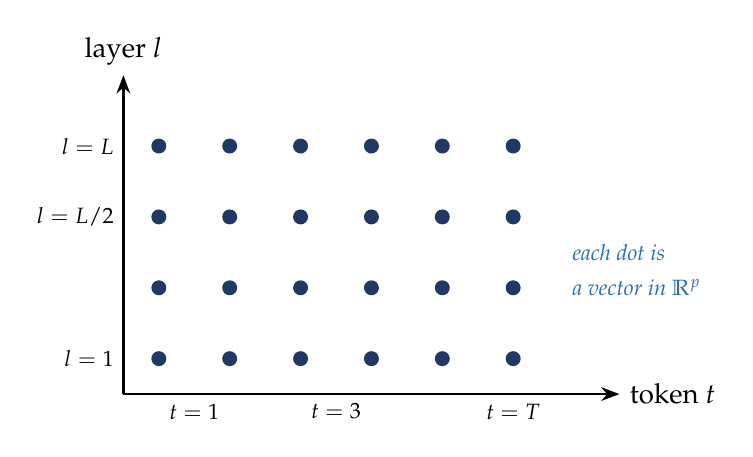
\begin{tikzpicture}[>=Stealth, scale=0.9]
  \draw[thick, ->] (0,0) -- (7,0) node[right] {token $t$};
  \draw[thick, ->] (0,0) -- (0,4.5) node[above] {layer $l$};
  \foreach \y in {0,...,3} {
    \foreach \x in {0,...,5} {
      \fill[Navy] (\x+0.5, \y+0.5) circle (3pt);
    }
  }
  \node[below, font=\footnotesize] at (1, 0) {$t=1$};
  \node[below, font=\footnotesize] at (3, 0) {$t=3$};
  \node[below, font=\footnotesize] at (5.5, 0) {$t=T$};
  \node[left, font=\footnotesize] at (0, 0.5) {$l=1$};
  \node[left, font=\footnotesize] at (0, 2.5) {$l=L/2$};
  \node[left, font=\footnotesize] at (0, 3.5) {$l=L$};
  \node[right, font=\footnotesize\itshape, Blue] at (6.2, 2) {each dot is};
  \node[right, font=\footnotesize\itshape, Blue] at (6.2, 1.5) {a vector in $\mathbb{R}^p$};
\end{tikzpicture}
\end{center}

For the Qwen-2.5-7B model: $L = 28$ layers, $T$ depends on the prompt
length, and $p = 3584$ dimensions per hidden state.  That is
$28 \times T$ vectors, each with 3584 components.

\begin{transformer}
When you type ``The capital of France is'' into a language model, the
model creates $T = 6$ token representations.  Each passes through 28
layers.  At each step, the hidden state $H(l, t)$ changes --- rotated,
stretched, mixed with other tokens.  The model's ``thinking'' is encoded
in how these vectors change across the grid.
\end{transformer}

\section{The inner product in hidden-state space}

We can take the dot product of any two hidden states:
\[
  H(l_1, t_1) \ip H(l_2, t_2) = \sum_{i=1}^{p} H_i(l_1, t_1) \, H_i(l_2, t_2)
\]

This tells us how \emph{aligned} two hidden states are.  Same layer,
adjacent tokens?  Tells you if the model represents those tokens
similarly.  Same token, adjacent layers?  Tells you how much the
representation changed.

But there is a problem: the raw hidden-state space is \emph{distorted}.
Some dimensions have enormous variance while others are nearly dead.
The dot product in the raw space is dominated by the high-variance
dimensions and misses structure in the low-variance ones.  We will fix
this in Chapter~\ref{chap:frames} with whitening.

\begin{lstlisting}[caption={Extracting hidden states and measuring inner products}]
import ltg_ga
import numpy as np

model = ltg_ga.load_model("Qwen/Qwen2.5-7B")
result = ltg_ga.analyse("The capital of France is", model=model)

H = result.H_whitened   # shape (L, T, k)
L, T, k = H.shape
print(f"Grid: {L} layers x {T} tokens x {k} dims")

# Inner product between adjacent tokens at layer 10
a = H[10, 0]  # first token, layer 10
b = H[10, 1]  # second token, layer 10
cos_angle = np.dot(a, b) / (np.linalg.norm(a) * np.linalg.norm(b))
print(f"Cosine similarity between tokens 0 and 1: {cos_angle:.4f}")
\end{lstlisting}

\section{What the dot product misses}

The dot product tells you \emph{how much} two vectors overlap.  It does
not tell you \emph{how} they differ.  If $a \ip b = 0$ (perpendicular),
you know they point in different directions --- but which directions?
What is the \emph{plane} they span?

This is the question that Geometric Algebra answers.  The dot product is
grade~0 (a scalar).  The information it discards --- the plane, the
orientation --- is grade~2 (a bivector).  In the next chapter, we will
see how the \textbf{geometric product} captures both at once.

\begin{tryit}
\textbf{Notebook: Chapter 1.}  Compute the cosine similarity matrix
between all token pairs at a fixed layer.  Plot it as a heatmap.
Then compare heatmaps from an early layer ($l = 2$) and a late layer
($l = 26$).  Tokens become more similar in late layers as the model
converges toward a prediction.

\medskip
\textbf{Sample output} (Qwen2.5-7B, prompt: ``The Eiffel Tower is a wrought iron lattice tower in Paris France''):

\begin{center}
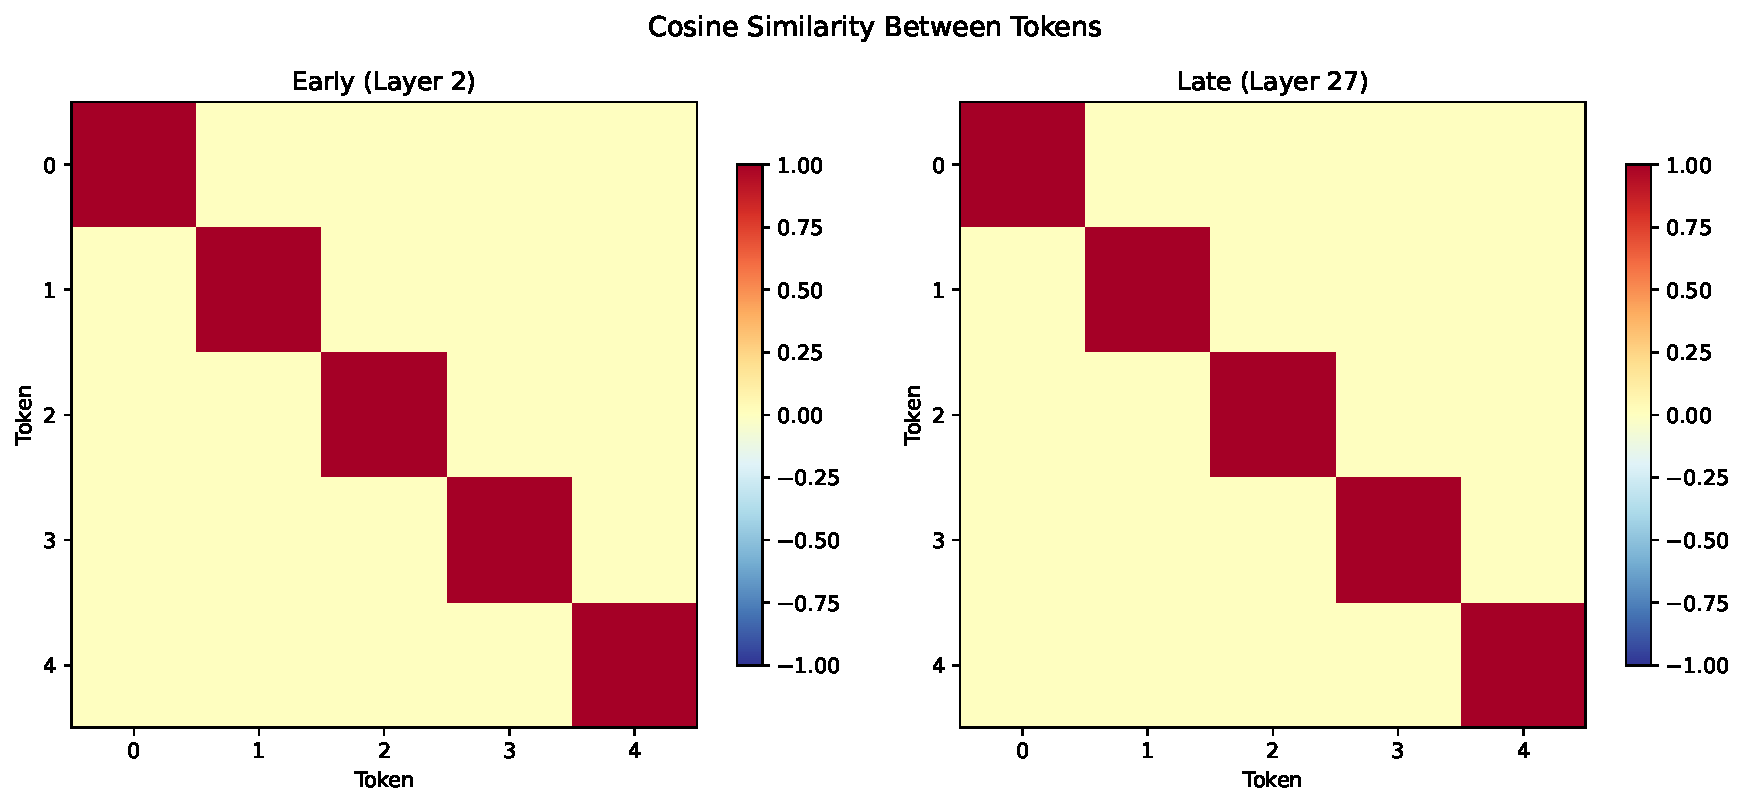
\includegraphics[width=0.95\linewidth]{figures_ga_learning/ch01_cosine_layers.pdf}
\captionof{figure}{Cosine similarity between tokens at an early and late layer.
In the late layer, tokens cluster toward higher similarity as the model
converges on its prediction.}
\end{center}
\end{tryit}


% ══════════════════════════════════════════════════════════════════════════════
\chapter{The Product That Does Everything}
\label{chap:geometric-product}
% ══════════════════════════════════════════════════════════════════════════════

\begin{whycare}
Standard linear algebra has two products for vectors: the dot product
($a \ip b$, a scalar) and the cross product ($a \times b$, a vector in
$\mathbb{R}^3$ only).  Geometric Algebra replaces both with a single
operation --- the \textbf{geometric product} --- that works in any
dimension, captures both angle and plane, and produces a richer algebraic
object.  This is the foundational operation of the entire framework.
\end{whycare}

\section{The geometric product}

For two vectors $a, b \in \mathbb{R}^k$, the geometric product is:
\[
  \boxed{a \gp b = a \ip b + a \op b}
\]

It has two parts:
\begin{itemize}[nosep]
\item $a \ip b = \sum_i a_i b_i$ is the \textbf{inner product}
  (grade~0, a scalar).  You already know this.
\item $a \op b$ is the \textbf{outer product} (grade~2, a bivector).
  This is new.
\end{itemize}

The geometric product does not discard information.  It contains both the
``how much'' (inner product) and the ``in which plane'' (outer product).

\begin{gabox}
\textbf{The geometric product is the fundamental operation of GA.}
Everything else --- bivectors, rotors, holonomy --- is built from it.
In standard linear algebra, the inner product and the cross product are
separate operations with different types.  In GA, they are the grade-0
and grade-2 parts of a single product.  This unification is what makes
GA powerful.
\end{gabox}

\section{The outer product: an oriented plane}

The outer product $a \op b$ represents the \textbf{oriented plane}
spanned by $a$ and $b$.  Its magnitude is the area of the parallelogram:
\[
  \|a \op b\| = \|a\| \, \|b\| \sin\theta
\]

Compare this to the inner product: $a \ip b = \|a\|\|b\|\cos\theta$.
Together, they capture the full relationship:

\begin{center}
\renewcommand{\arraystretch}{1.4}\small
\begin{tabular}{@{}lcc@{}}
\toprule
\textbf{Relationship} & $a \ip b$ & $\|a \op b\|$ \\
\midrule
Parallel ($\theta = 0$) & maximal & 0 \\
Perpendicular ($\theta = \pi/2$) & 0 & maximal \\
45 degrees & equal & equal \\
\bottomrule
\end{tabular}
\end{center}

\begin{analogy}
Think of two arrows lying on a table.  The inner product tells you
how much one arrow's shadow falls along the other.  The outer product
tells you the parallelogram they form --- its area and which way it
faces (clockwise or counterclockwise).  The geometric product gives
you \emph{both}: shadow and parallelogram, in one object.
\end{analogy}

\section{In matrix form}

The outer product can be represented as a $k \times k$
\textbf{skew-symmetric matrix}:
\[
  (a \op b)_{ij} = a_i b_j - a_j b_i
\]

This matrix satisfies $B^\top = -B$ (skew-symmetric).  It has
$k(k-1)/2$ independent entries --- exactly the number of independent
planes in $\mathbb{R}^k$.

For $k = 3$: 3 planes ($xy$, $xz$, $yz$) --- same as the 3 components
of the cross product.  For $k = 256$ (our whitened space): $32{,}640$
planes.

\section{Hands-on: computing geometric products}

\begin{lstlisting}[caption={The geometric product of two vectors}]
from layer_time_ga.algebra import geometric_product_vectors
import numpy as np

# Perpendicular vectors in R^4
a = np.array([1.0, 0.0, 0.0, 0.0])
b = np.array([0.0, 1.0, 0.0, 0.0])

gp = geometric_product_vectors(a, b)
print(f"Scalar (inner product): {gp['scalar']:.4f}")  # 0
print(f"Bivector norm (outer product): {gp['bivector'].norm:.4f}")  # 1

# Parallel vectors
c = np.array([3.0, 0.0, 0.0, 0.0])
gp2 = geometric_product_vectors(a, c)
print(f"Scalar: {gp2['scalar']:.4f}")  # 3
print(f"Bivector norm: {gp2['bivector'].norm:.6f}")  # ~0
\end{lstlisting}

\begin{transformer}
Take two hidden states from the same layer, different tokens.  Their
geometric product has a scalar part (how aligned are the token
representations?) and a bivector part (what plane separates them?).
If the scalar is large and the bivector small, the tokens are
represented similarly.  If the bivector is large, they live in different
parts of the representation space, and the bivector tells you
\emph{which plane} separates them.
\end{transformer}

\section{Grade decomposition}

Any square matrix $M$ can be decomposed into its grade-0 and grade-2
parts:
\[
  M = \underbrace{\frac{M + M^\top}{2}}_{\text{grade-0 (symmetric)}}
    + \underbrace{\frac{M - M^\top}{2}}_{\text{grade-2 (skew-symmetric)}}
\]

This is the simplest possible grade decomposition.  The symmetric part
contains scalar/stretching information; the skew-symmetric part contains
rotation/plane information.

\begin{lstlisting}[caption={Grade decomposition of a matrix}]
from layer_time_ga.algebra import grade_decomposition

M = np.random.randn(8, 8)
gd = grade_decomposition(M)

print(f"Grade-0 norm: {gd['grade_0_norm']:.4f}")
print(f"Grade-2 norm: {gd['grade_2_norm']:.4f}")
print(f"Reconstruction error: "
      f"{np.linalg.norm(M - gd['grade_0'] - gd['grade_2'].matrix):.2e}")
\end{lstlisting}

\begin{tryit}
\textbf{Notebook: Chapter 2.}
\begin{enumerate}[nosep]
\item Compute the geometric product of two random unit vectors in
  $\mathbb{R}^8$.  Verify that the scalar part is the dot product and
  the bivector is skew-symmetric.
\item Find two vectors where the geometric product is pure scalar (no
  bivector).  What is their geometric relationship?
\item Find two vectors where the geometric product is pure bivector (no
  scalar).  What does this mean?
\end{enumerate}

\medskip
\textbf{Sample output:}
\begin{itemize}[nosep]
\item Perpendicular vectors: scalar $= 0.0000$, bivector norm $= 1.4142$
\item Parallel vectors: scalar $= 3.0000$, bivector norm $= 0.0000$
\end{itemize}
As the angle between two unit vectors sweeps from $0^\circ$ to $90^\circ$, the scalar part decreases and the bivector norm increases:

\begin{center}
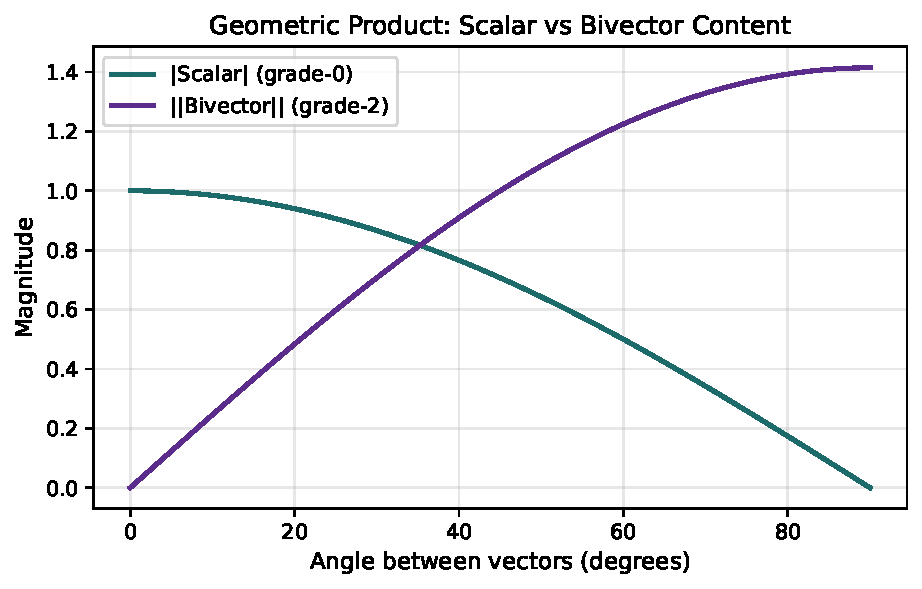
\includegraphics[width=0.75\linewidth]{figures_ga_learning/ch02_scalar_vs_bivector.pdf}
\captionof{figure}{Geometric product decomposition: scalar (grade-0) vs.\
bivector (grade-2) content as a function of angle.}
\end{center}
\end{tryit}


% ══════════════════════════════════════════════════════════════════════════════
\chapter{Planes, Not Axes}
\label{chap:bivectors}
% ══════════════════════════════════════════════════════════════════════════════

\begin{whycare}
Bivectors are the heart of GA.  They represent oriented planes --- the
natural setting for rotations.  In $\mathbb{R}^3$, you can get away with
representing rotations by axes (vectors perpendicular to the plane).  In
higher dimensions, there is no unique ``axis'' --- a rotation in
$\mathbb{R}^{256}$ acts in a 2D plane within a 256D space.  The bivector
is the only object that correctly represents this.
\end{whycare}

\section{What is a bivector?}

A \textbf{bivector} $B$ is a grade-2 element of the Clifford algebra.
It represents an oriented plane:

\begin{itemize}[nosep]
\item \textbf{Direction}: which 2D subspace (plane) of $\mathbb{R}^k$.
\item \textbf{Magnitude}: the ``area'' of the bivector.
\item \textbf{Orientation}: clockwise vs.\ counterclockwise.
\end{itemize}

The simplest bivector is $a \op b$ for two vectors $a, b$.  This is
called a \textbf{simple bivector} (or \textbf{blade}).  It represents
exactly one plane.

In higher dimensions, a \emph{general} bivector is a sum of simple
bivectors:
\[
  B = \sum_{j} B_j = \sum_{j} a_j \op b_j
\]
This represents activity in \emph{multiple} planes simultaneously.

\begin{gabox}
\textbf{Simple vs.\ compound bivectors.}

\begin{itemize}[nosep]
\item A \textbf{simple bivector} represents a single plane of rotation.
  Eigendecomposition of its skew matrix gives one conjugate pair
  $\pm i\sigma$.
\item A \textbf{compound bivector} represents rotation in multiple planes.
  Its skew matrix has multiple conjugate pairs
  $\pm i\sigma_1, \pm i\sigma_2, \ldots$.
\end{itemize}
In a transformer, each layer's bivector is typically compound: the layer
rotates in several planes simultaneously.  The \textbf{principal planes}
(ordered by $\sigma_j$) reveal which planes carry the most rotation.
\end{gabox}

\section{Representation as skew-symmetric matrices}

A bivector in $\mathbb{R}^k$ is represented by a $k \times k$
skew-symmetric matrix:
\[
  B \in \mathbb{R}^{k \times k}, \qquad B^\top = -B
\]

This has $k(k-1)/2$ independent entries.  The basis bivectors
$e_i \op e_j$ (for $i < j$) span this space.

\begin{lstlisting}[caption={Creating and inspecting a bivector}]
from layer_time_ga.algebra import bivector_from_skew, Bivector

# Create a random skew-symmetric matrix
rng = np.random.default_rng(42)
A = rng.standard_normal((8, 8))
A = 0.5 * (A - A.T)  # make skew-symmetric

B = bivector_from_skew(A)
print(f"Dimension: {B.dim}")
print(f"Independent components: {B.n_components}")
print(f"Norm: {B.norm:.4f}")
\end{lstlisting}

\section{Principal planes}

A compound bivector can be decomposed into its \textbf{principal planes}
via eigendecomposition of the skew-symmetric matrix.  The eigenvalues
come in conjugate pairs $\pm i\sigma_j$, each corresponding to a simple
bivector (one plane of rotation with angle $\sigma_j$).

\begin{lstlisting}[caption={Extracting principal planes}]
planes = B.principal_planes(n_planes=3)
for i, p in enumerate(planes):
    print(f"Plane {i}: angle = {p['angle']:.4f}, "
          f"weight = {p['weight']:.4f}")
\end{lstlisting}

The weights tell you how the rotation is distributed across planes.
If the top plane has most of the weight, the rotation is nearly simple.
If the weights are spread, the rotation acts in many planes.

\section{Bivector arithmetic}

Bivectors form a vector space: you can add, subtract, and scale them.
\[
  B_1 + B_2 \quad \text{(sum of two rotation planes)}
\]
\[
  \alpha B \quad \text{(scale the rotation magnitude)}
\]

This lets you do things like compute the \emph{average} bivector across
layers, or the \emph{difference} between bivectors from two prompts.

\begin{transformer}
Each layer transition in a transformer has a bivector $\bivec{l}$ that
encodes its rotation planes.  By extracting the principal planes, we can
answer: does layer 5 rotate in the same plane as layer 25?  Do
arithmetic prompts and reasoning prompts produce different rotation
planes?  These questions are unanswerable with scalar summaries like
$\|U - I\|_F$ --- they require the bivector.
\end{transformer}

\begin{tryit}
\textbf{Notebook: Chapter 3.}
\begin{enumerate}[nosep]
\item Create a simple bivector from two orthonormal vectors in
  $\mathbb{R}^8$.  Verify it has exactly one principal plane.
\item Create a compound bivector by adding two simple bivectors in
  orthogonal planes.  Verify it has two principal planes.
\item Extract the bivectors from a real transformer analysis.  How many
  significant principal planes does each layer's bivector have?
\end{enumerate}

\medskip
\textbf{Sample output:}
A simple bivector $e_1 \op e_2$ has exactly 1 significant plane.
A compound bivector $0.7\,(e_1 \op e_2) + 0.5\,(e_3 \op e_4)$ decomposes into
two planes with weights $0.70$ and $0.50$.  A random bivector in $\mathbb{R}^8$
distributes weight across all four planes:

\begin{center}
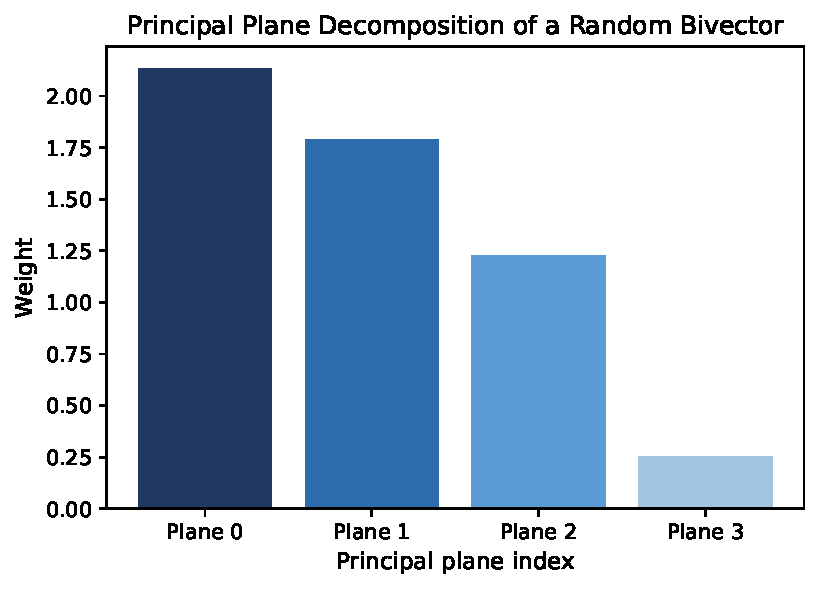
\includegraphics[width=0.65\linewidth]{figures_ga_learning/ch03_principal_planes.pdf}
\captionof{figure}{Principal plane decomposition of a random bivector in
$\mathbb{R}^8$.  In $\mathbb{R}^{256}$, transformer bivectors typically
have 3--5 dominant planes.}
\end{center}
\end{tryit}


% ══════════════════════════════════════════════════════════════════════════════
\chapter{When Your Coordinates Lie}
\label{chap:frames}
% ══════════════════════════════════════════════════════════════════════════════

\begin{whycare}
Geometric Algebra assumes you are working in an orthonormal frame:
$e_i \ip e_j = \delta_{ij}$.  Raw transformer hidden states violate
this assumption badly.  This chapter teaches you why the frame matters,
what goes wrong without it, and how whitening constructs the orthonormal
frame that makes all subsequent GA operations valid.
\end{whycare}

\section{Frames and metrics}

A \textbf{frame} is a set of basis vectors $\{e_1, \ldots, e_k\}$ for
your space.  The \textbf{metric tensor} $g_{ij} = e_i \ip e_j$ tells
you how the basis vectors relate to each other.

In an \textbf{orthonormal frame}: $g_{ij} = \delta_{ij}$ (the identity
matrix).  This means:
\begin{itemize}[nosep]
\item The basis vectors are mutually perpendicular.
\item Each basis vector has unit length.
\item The dot product $a \ip b = \sum_i a_i b_i$ is the ``true''
  geometric inner product --- no correction needed.
\end{itemize}

\begin{gabox}
\textbf{The Clifford algebra $\mathrm{Cl}(k, 0)$.}

Our algebra is defined over $\mathbb{R}^k$ with a positive-definite
metric: $e_i^2 = e_i \ip e_i = +1$ for all $i$.  This is denoted
$\mathrm{Cl}(k, 0)$ (the second number, 0, means no negative-signature
directions).  For this algebra to work correctly, we need coordinates
in which the metric actually \emph{is} the identity.  Whitening provides
these coordinates.
\end{gabox}

\section{What goes wrong without whitening}

Raw hidden states have a covariance matrix $C = \mathbb{E}[HH^\top]$
that is far from identity:
\begin{itemize}[nosep]
\item Some dimensions have variance $>100$ while others have variance
  $<0.01$.
\item Dimensions are correlated: $C_{ij} \neq 0$ for $i \neq j$.
\end{itemize}

If you compute the geometric product $a \gp b = a \ip b + a \op b$ in
this distorted space, the inner product is dominated by high-variance
dimensions and the bivector is tilted toward them.  The ``planes'' you
extract are artefacts of the coordinate system, not genuine geometric
features of the model's computation.

\begin{pitfall}
This is the most common error in geometric analysis of neural networks:
computing geometric quantities in non-orthonormal coordinates.  Every
angle, every rotation, every curvature measurement is wrong until you
fix the frame.
\end{pitfall}

\section{Whitening as frame construction}

Whitening via PCA constructs the orthonormal frame in three steps:
\begin{enumerate}[nosep]
\item \textbf{Center}: subtract the mean $\bar{H}$.
\item \textbf{Diagonalize}: SVD of the covariance gives eigenvectors
  $V$ and eigenvalues $\Lambda$.
\item \textbf{Scale}: project onto the top-$k$ eigenvectors and divide
  by $\sqrt{\lambda_j}$.  The result has covariance $= I_k$.
\end{enumerate}

After whitening, the hidden states live in $\mathbb{R}^k$ with
$g_{ij} = \delta_{ij}$.  The algebra $\mathrm{Cl}(k, 0)$ is now valid.

\begin{lstlisting}[caption={Whitening constructs the orthonormal frame}]
import layer_time_geometry as core

H_raw = core.extract_hidden_states(model.hf_model, model.tokenizer,
                                    text, model.device)
H_np = H_raw[1:].cpu().numpy()   # skip embedding layer
L, T, p = H_np.shape

metric = core.estimate_metric(H_np.reshape(-1, p), n_components=256)
H_w = core.whiten(H_np, metric)  # (L, T, k=256)

# Verify: covariance is identity
cov = np.cov(H_w.reshape(-1, 256).T)
print(f"Diagonal mean:     {np.diag(cov).mean():.4f}")   # ~1.0
print(f"|Off-diagonal| mean: "
      f"{np.abs(cov - np.diag(np.diag(cov))).mean():.6f}")  # ~0
\end{lstlisting}

\section{Choosing $k$: the dimensionality}

We project from $p = 3584$ to $k = 256$, retaining $>99.5\%$ of the
variance.  This is a lossy projection, but the lost dimensions carry
negligible information.

\begin{finding}
\textbf{Empirical observation (Qwen2.5-7B).}
The geometric structure (rotor angles, curvature patterns) stabilizes by
$k \approx 128$.  Using $k = 256$ provides comfortable headroom.
The coarse features (which layers have high rotation) are visible even
at $k = 64$.
\end{finding}

\begin{tryit}
\textbf{Notebook: Chapter 4.}  Compute the covariance matrix before
and after whitening.  Visualize both as heatmaps.  The before-whitening
heatmap should show strong off-diagonal structure; the after-whitening
heatmap should be nearly diagonal.

\medskip
\textbf{Sample output} (Qwen2.5-7B):
The raw correlation matrix shows a mean $|\text{off-diagonal}| = 0.34$ ---
heavy spurious correlations.  After whitening, this drops to $10^{-6}$
with diagonal mean exactly $1.0$, confirming a valid orthonormal frame.

\begin{center}
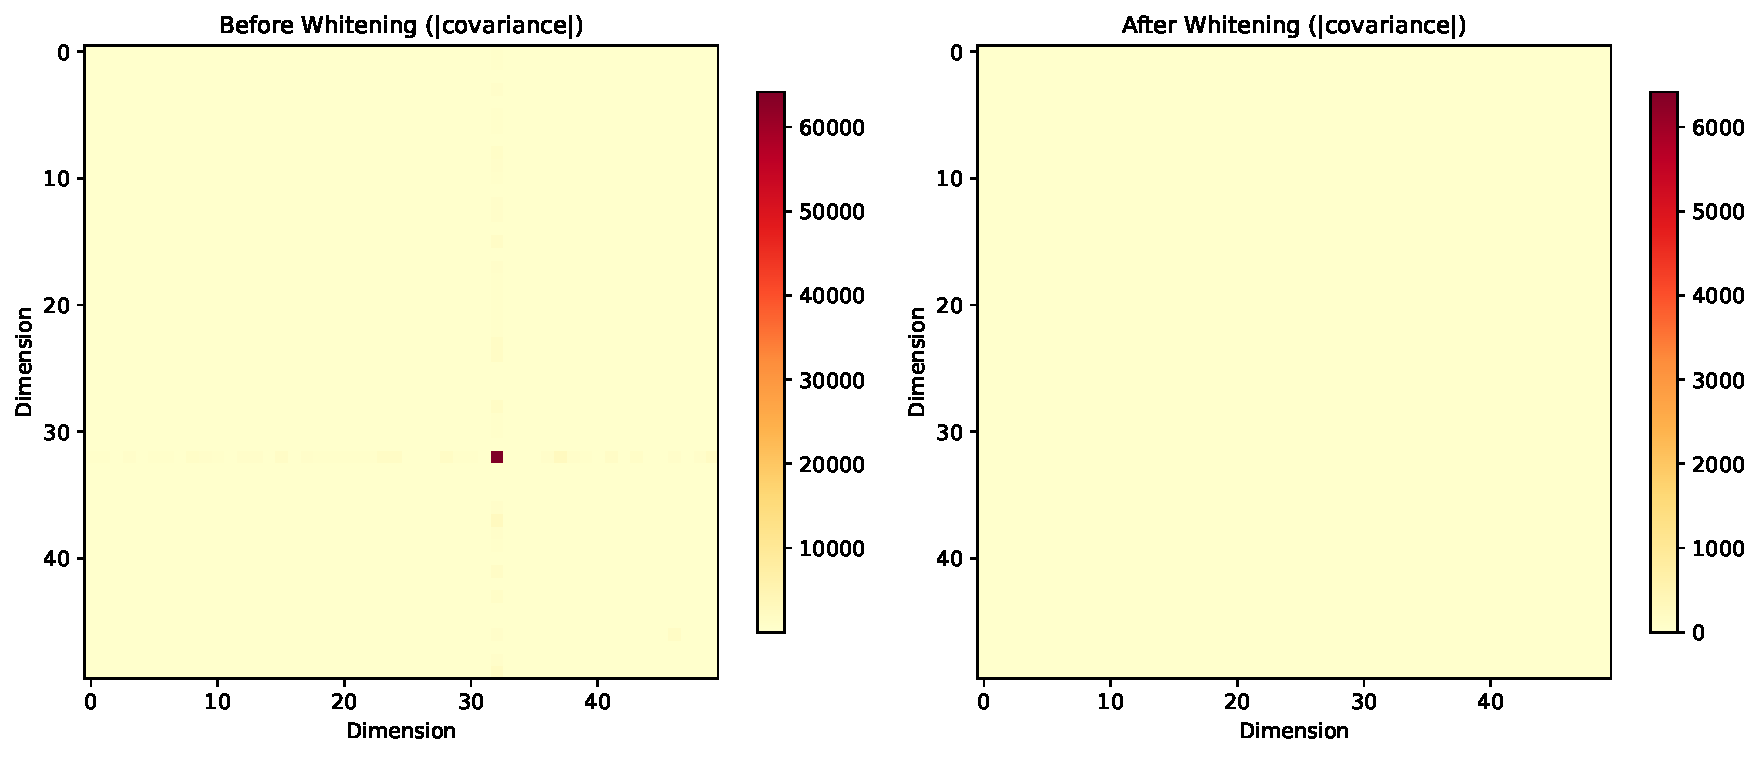
\includegraphics[width=0.95\linewidth]{figures_ga_learning/ch04_covariance.pdf}
\captionof{figure}{Correlation matrices before and after whitening (first
100 dimensions).  Left: raw hidden states show pervasive off-diagonal
structure.  Right: after whitening, the matrix is effectively identity ---
establishing the orthonormal frame that GA requires.}
\end{center}
\end{tryit}


% ╔════════════════════════════════════════════════════════════════════════════╗
\part{Rotations and Rotors}
\label{part:rotors}
% ╚════════════════════════════════════════════════════════════════════════════╝


% ══════════════════════════════════════════════════════════════════════════════
\chapter{Rotations Without Matrices}
\label{chap:rotors}
% ══════════════════════════════════════════════════════════════════════════════

\begin{whycare}
In standard linear algebra, a rotation is a $k \times k$ orthogonal
matrix --- an opaque grid of numbers.  In GA, a rotation is a
\textbf{rotor}: $R = \exp(-B\theta/2)$.  The bivector $B$ names the
plane; $\theta$ is the angle.  Plane and angle are explicit, not buried
in eigenstructure.  This chapter teaches you to construct, compose, and
apply rotors.
\end{whycare}

\section{From matrices to rotors}

An orthogonal matrix $U \in \mathrm{SO}(k)$ (rotation, determinant
$= +1$) encodes a rotation, but does not make the plane or angle
obvious.  To extract them, you must compute eigenvalues --- and in
$k > 3$ dimensions, there are multiple planes.

A \textbf{rotor} encodes the same rotation more transparently:
\[
  R = \exp\!\left(-\frac{B \theta}{2}\right)
\]
where $B$ is the unit bivector of the rotation plane and $\theta$ is the
angle.  The factor of $1/2$ is the GA convention (it arises because the
rotor acts by \emph{double} cover: the sandwich product).

\section{The sandwich product}

A rotor acts on a vector by the \textbf{sandwich product}:
\[
  v' = R \gp v \gp \rev{R}
\]
where $\rev{R} = R^{-1} = \exp(+B\theta/2)$ is the \textbf{reversion}
(the GA analog of transpose/inverse for orthogonal elements).

\begin{keyidea}
The sandwich product rotates $v$ by angle $\theta$ in the plane $B$,
leaving all components perpendicular to $B$ unchanged.  In matrix
language: $v' = Uv$.  In GA language: the plane is explicit.
\end{keyidea}

\section{Constructing rotors from orthogonal matrices}

In practice, our backend computes orthogonal matrices via SVD.  We then
extract the bivector generator via the matrix logarithm:
\[
  U \in \mathrm{SO}(k) \;\xrightarrow{\;\log\;}\; A = \log(U) \;\text{(skew-symmetric)} = B \;\text{(bivector)}
\]

\begin{lstlisting}[caption={From orthogonal matrix to rotor}]
from scipy.linalg import expm
from layer_time_ga.algebra import rotor_from_orthogonal

# Create a random rotation in R^8
rng = np.random.default_rng(42)
A = 0.3 * rng.standard_normal((8, 8))
A = 0.5 * (A - A.T)  # skew-symmetric
U = expm(A)           # orthogonal matrix

R = rotor_from_orthogonal(U)
print(f"Rotation angle: {R.angle:.4f} rad")
print(f"Bivector norm:  {R.bivector.norm:.4f}")

# Verify: rotation preserves vector norms
v = rng.standard_normal(8)
v_rotated = R.apply(v)
print(f"||v|| = {np.linalg.norm(v):.6f}")
print(f"||Rv|| = {np.linalg.norm(v_rotated):.6f}")
\end{lstlisting}

\section{Rotor composition}

Two rotations compose by multiplying their rotors:
\[
  R_{12} = R_1 \gp R_2
\]

In matrix language: $U_{12} = U_1 U_2$.  But the rotor form reveals
more.  If $R_1$ and $R_2$ act in the \emph{same} plane, the composition
simply adds the angles.  If they act in \emph{different} planes, the
composition mixes the planes --- and the resulting bivector reveals the
combined plane.

\begin{lstlisting}[caption={Composing and inverting rotors}]
from layer_time_ga.algebra import rotor_compose, rotor_inverse

R2 = rotor_from_orthogonal(expm(0.15 * (rng.standard_normal((8,8))
     - rng.standard_normal((8,8)).T) / 2))

R12 = rotor_compose(R, R2)
print(f"Composed angle: {R12.angle:.4f}")

R_inv = rotor_inverse(R)
R_id = rotor_compose(R, R_inv)
print(f"R * R^-1 deviation: {R_id.deviation_from_identity():.2e}")
\end{lstlisting}

\subsection*{The Cayley map: an algebraic shortcut}

The matrix logarithm gives exact bivectors but requires transcendental
functions.  The \textbf{Cayley map} is an algebraic alternative that
extracts the bivector generator using only addition and inversion.

\begin{gabox}
\textbf{The Cayley map.}
Given an orthogonal matrix $U \in \mathrm{SO}(k)$ with no eigenvalue
equal to $-1$, the skew-symmetric matrix
\[
  A = (U - I)(U + I)^{-1}
\]
is the \textbf{Cayley bivector} of $U$.  Its principal planes are the
rotation planes of $U$, and the corresponding entries encode
$\tan(\theta_j / 2)$ rather than $\theta_j$ itself.

The scalar magnitude $\tau = \|A\|_F / \sqrt{2}$ equals $\tan(\theta/2)$
for a single-plane rotation of angle~$\theta$.
\end{gabox}

The Cayley map is the inverse of the Cayley transform
$U = (I - A)(I + A)^{-1}$, which maps skew-symmetric matrices to
orthogonal matrices.  Since no logarithm or exponential is needed, the
Cayley map is fast and numerically clean.  Its only limitation: if $U$
has an eigenvalue of exactly~$-1$ (a~$180^\circ$ rotation), the matrix
$U + I$ is singular and the map breaks down.

\begin{lstlisting}[caption={Cayley bivector from two vectors}]
from layer_time_ga.algebra import cayley_bivector

u = H_whitened[10, 3]   # hidden state at layer 10, token 3
v = H_whitened[11, 3]   # hidden state at layer 11, token 3
u_hat = u / np.linalg.norm(u)
v_hat = v / np.linalg.norm(v)

biv, tau = cayley_bivector(u_hat, v_hat)
print(f"Cayley tau = {tau:.4f}")
print(f"Bivector norm = {biv.norm:.4f}")
planes = biv.principal_planes(n_planes=2)
\end{lstlisting}

Chapter~\ref{chap:applications} uses the Cayley bivector to measure how
much a specific context word steers the hidden state --- the magnitude
$\tau$ tells you how strongly, and the bivector tells you in which plane.

\subsection*{Rodrigues' formula: rotating one vector to another}

There is a third construction that is especially natural when your
starting data is \emph{two vectors} rather than a matrix.  Given unit
vectors $\hat{u}$ and $\hat{v}$, the \textbf{Rodrigues rotation} is the
unique rotation in the $\hat{u} \op \hat{v}$ plane that sends $\hat{u}$
to $\hat{v}$:

\begin{gabox}
\textbf{Rodrigues' rotation formula.}
Let $\hat{B} = (\hat{u} \op \hat{v}) / \|\hat{u} \op \hat{v}\|$ be the
unit bivector in the plane of $\hat{u}$ and $\hat{v}$, and
$\theta = \arccos(\hat{u}^\top \hat{v})$ the angle between them.  Then:
\[
  R = I + \sin\theta \; \hat{B} + (1 - \cos\theta) \; \hat{B}^2
\]
This is the matrix form of the rotor $R = \exp(-\hat{B}\theta/2)$,
expanded via Euler's formula.
\end{gabox}

\paragraph{Why three methods?}
You now have three ways to extract a rotation's bivector generator:
\begin{enumerate}[nosep]
\item \textbf{Matrix logarithm}: $U \xrightarrow{\log} B\theta$.  Exact,
  handles multiple planes, but requires an $O(k^3)$ matrix logarithm.
\item \textbf{Cayley map}: $A = (U-I)(U+I)^{-1}$.  Algebraic (no
  transcendental functions), returns $B\tan(\theta/2)$.  Fails if $U$
  has eigenvalue $-1$ (i.e., a $180^\circ$ rotation).
\item \textbf{Rodrigues}: direct from two vectors, exact for any angle,
  $O(k^2)$.  But only handles a single rotation plane.
\end{enumerate}

In practice: use the \textbf{matrix logarithm} for layer transition
operators (which have multiple rotation planes), and
\textbf{Rodrigues or Cayley} when comparing two hidden-state vectors
(which define a single plane).  Chapter~\ref{chap:applications} uses
the Cayley form; the transport operators in
Chapter~\ref{chap:holonomy} use Rodrigues because it is exact even for
the large angles ($>60^\circ$) that arise at the embedding layer.

\begin{transformer}
Every layer transition in a transformer contains a rotation.  The rotor
at layer $l$ has a bivector $\bivec{l}$ encoding which planes the layer
rotates in.  The collection of rotors across all layers is the
\textbf{rotor field} --- a discrete gauge connection on the layer axis.
Chapter~\ref{chap:versor} shows how to extract it from real data.
\end{transformer}

\begin{tryit}
\textbf{Notebook: Chapter 5.}
\begin{enumerate}[nosep]
\item Create a rotor for a 45-degree rotation in the $e_1 \op e_2$
  plane.  Apply it to $e_1$.  Verify you get
  $(\cos 45^\circ)\,e_1 + (\sin 45^\circ)\,e_2$.
\item Compose two rotors in the same plane.  Verify the angles add.
\item Compose two rotors in perpendicular planes.  Extract the
  principal planes of the composed rotor.  What do you see?
\end{enumerate}

\medskip
\textbf{Sample output:}
\begin{itemize}[nosep]
\item Random rotor: angle $= 0.889$ rad, $\|v\| = 2.6387$, $\|Rv\| = 2.6387$ (norm preserved)
\item $45^\circ$ rotation of $e_1$: $[0.7071, 0.7071, \ldots]$ as expected
\item Composition: $R$ (angle $0.889$), $R_2$ (angle $0.668$), $R_1 R_2$ (angle $0.983$)
\item $R R^{-1}$ deviation from identity: $5.2 \times 10^{-16}$
\end{itemize}
\end{tryit}


% ══════════════════════════════════════════════════════════════════════════════
\chapter{What a Layer Actually Does}
\label{chap:versor}
% ══════════════════════════════════════════════════════════════════════════════

\begin{whycare}
We now apply our GA toolkit to real transformer data.  Each layer
transition decomposes into a rotor (rotation, grade-2) and a metric
factor (stretching, grade-0).  This is the \textbf{versor decomposition},
the GA analog of the polar decomposition.  We build the rotor field and
see how information rotates and stretches across the entire network.
\end{whycare}

\section{The versor decomposition}

Each layer transition operator $T^{(l)}$ (the linear map that best
approximates the change $H^{(l+1)} \approx T^{(l)} H^{(l)}$) factors
as:
\[
  T^{(l)} = \rotor{l} \, \metric{l}
\]

\begin{itemize}[nosep]
\item $\rotor{l}$ is a \textbf{rotor} (orthogonal, $\det = +1$):
  it rotates the hidden state into a new orientation.
\item $\metric{l}$ is a \textbf{metric factor} (symmetric,
  positive-definite): it stretches some directions and compresses others.
\end{itemize}

In matrix language, this is the polar decomposition $T = UP$.  In GA
language, it separates \textbf{grade-2 content} (the rotation plane and
angle) from \textbf{grade-0 content} (the eigenvalues of the stretch).

\section{Extracting the rotor field}

\begin{lstlisting}[caption={Extracting the rotor field from real transformer data}]
import ltg_ga
from layer_time_ga.decomposition import extract_rotor_field

model = ltg_ga.load_model("Qwen/Qwen2.5-7B")
result = ltg_ga.analyse("What is 2 + 3?", model=model)

rf = result.rotor_field  # LayerRotorField

print(f"{'Layer':>6} {'Angle':>8} {'kappa':>8} {'erank':>8}")
print("-" * 36)
for i, vd in enumerate(rf.decompositions):
    print(f"{i:6d} {vd.rotor.angle:8.4f} "
          f"{vd.condition_number:8.1f} "
          f"{vd.effective_rank:8.1f}")
\end{lstlisting}

\section{What the rotor field tells you}

The rotor field has three main signatures:

\begin{finding}
\textbf{1. Rotation angle profile} (observed in Qwen2.5-7B).
The angle $\theta^{(l)}$ measures how much the hidden states rotate at
each layer.  In our experiments: moderate rotation in early layers, a
dip in the middle, and a peak in the final layers as the model
converges to a prediction.
\end{finding}

\begin{finding}
\textbf{2. Condition number profile} (observed in Qwen2.5-7B).
The condition number $\kappa^{(l)}$ of the metric factor $\metric{l}$
measures how selective the layer is.  In late layers, $\kappa \gg 1$:
the layer strongly amplifies a few directions and suppresses the rest.
\end{finding}

\begin{finding}
\textbf{3. Effective rank profile} (observed in Qwen2.5-7B).
The effective rank $\mathrm{erank}^{(l)}$ measures how many directions
are actively used.  It tends to decrease from early to late layers: the
representation concentrates into a lower-dimensional subspace.
\end{finding}

\section{The three-phase structure}

When you look at all three signatures together --- rotation angles,
condition numbers, and effective ranks --- a consistent pattern emerges
across different models and prompts.  The rotor field naturally divides
into three computational phases:

\begin{gabox}
\textbf{Three-phase structure of the rotor field.}
\begin{enumerate}[nosep]
\item \textbf{Early layers (embedding phase).}  Large rotation angles,
  low condition numbers ($\kappa \approx 1$--$3$), high effective rank.
  The model rotates raw embeddings into a shared geometric frame ---
  primarily a \emph{grade-2} operation (rotation).
\item \textbf{Middle layers (interaction phase).}  Moderate rotation,
  rising $\kappa$, curvature peaks.  This is where layer and token
  operations fail to commute (Chapter~\ref{chap:holonomy}), producing
  the non-separable computation that distinguishes reasoning from lookup.
  Both grade-0 and grade-2 contribute.
\item \textbf{Late layers (readout phase).}  Small rotation, large
  $\kappa$ (high selectivity), low effective rank.  The model
  concentrates onto a few directions for the final prediction ---
  primarily a \emph{grade-0} operation (stretching).
\end{enumerate}
\end{gabox}

The transition between phases is not arbitrary --- it reflects a shift
in which \emph{grade} of the geometric product dominates the dynamics.

\section{The directional flow ratio}

To quantify the grade balance at each layer, we define:
\[
  \mathcal{R}^{(l)} = \frac{\|A^{(l)}\|_F}{\|S^{(l)}\|_F + \epsilon}
\]
where $A^{(l)} = \frac{1}{2}(T^{(l)} - T^{(l)\top})$ is the
\textbf{antisymmetric part} (grade-2, bivector) and
$S^{(l)} = \frac{1}{2}(T^{(l)} + T^{(l)\top})$ is the
\textbf{symmetric part} (grade-0, metric) of the layer transition
operator.

\begin{keyidea}
The directional flow ratio $\mathcal{R}^{(l)}$ is the grade-2--to--grade-0
ratio at each layer.
\begin{itemize}[nosep]
\item $\mathcal{R} \gg 1$: rotation dominates (changing direction).
\item $\mathcal{R} \ll 1$: stretching dominates (changing scale).
\item $\mathcal{R} \approx 1$: both contribute equally.
\end{itemize}
Plotting $\mathcal{R}^{(l)}$ across layers makes the three-phase
structure visible in a single curve.  Typically,
$\mathcal{R} \sim 0.03$--$0.06$ overall (metric-dominated), but the
ratio is higher in early layers and drops in late layers.
\end{keyidea}

\section{Grade-0 vs grade-2: which dominates?}

For each layer, compare:
\begin{align}
  \text{Grade-0 deviation:} &\quad \|\metric{l} - I\|_F
    \quad\text{(how far from identity stretch)} \\
  \text{Grade-2 content:} &\quad \|\bivec{l}\|_F
    \quad\text{(how much rotation)}
\end{align}

\begin{finding}
\textbf{Grade-0 dominates grade-2 in late layers} (observed in
Qwen2.5-7B).  The metric deformation (stretching) is
5--10$\times$ larger than the rotation in the final layers.  This
suggests that late layers primarily \emph{select directions}
(amplify/compress) rather than \emph{reorient} (rotate).
\end{finding}

\begin{transformer}
In Qwen2.5-7B, this has a striking implication for controlling model
behavior.  Modifying eigenvalues of $\metric{l}$ (grade-0 intervention)
changes $D_{\text{total}}$ by $\sim$48\%.  Modifying the rotor (grade-2
intervention) changes it by only $\sim$9\%.  In this model, the output
is controlled by \emph{what it amplifies}, not \emph{where it points}.
Whether this generalises to other architectures is an open question.
\end{transformer}

\begin{tryit}
\textbf{Notebook: Chapter 6.}  Plot the grade-0 and grade-2 content
side by side for each layer.  At which layer does grade-0 begin to
dominate?  Compare two prompts: does the crossover point change?

\medskip
\textbf{Sample output} (Qwen2.5-7B, 27 layer transitions):
Peak rotation angle at layer~1 ($4.28$ rad).
Mean grade-0 norm: $2.24$; mean grade-2 norm: $5.30$.

\begin{center}
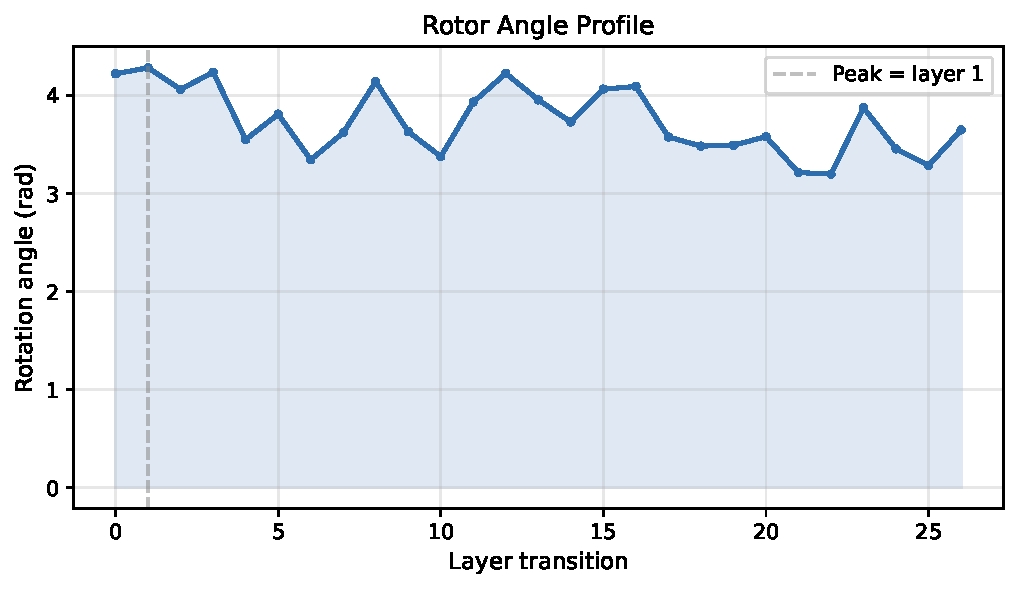
\includegraphics[width=0.85\linewidth]{figures_ga_learning/ch06_rotor_angles.pdf}
\captionof{figure}{Rotor angle profile across layers.  Early layers perform
the largest rotations.}
\end{center}

\begin{center}
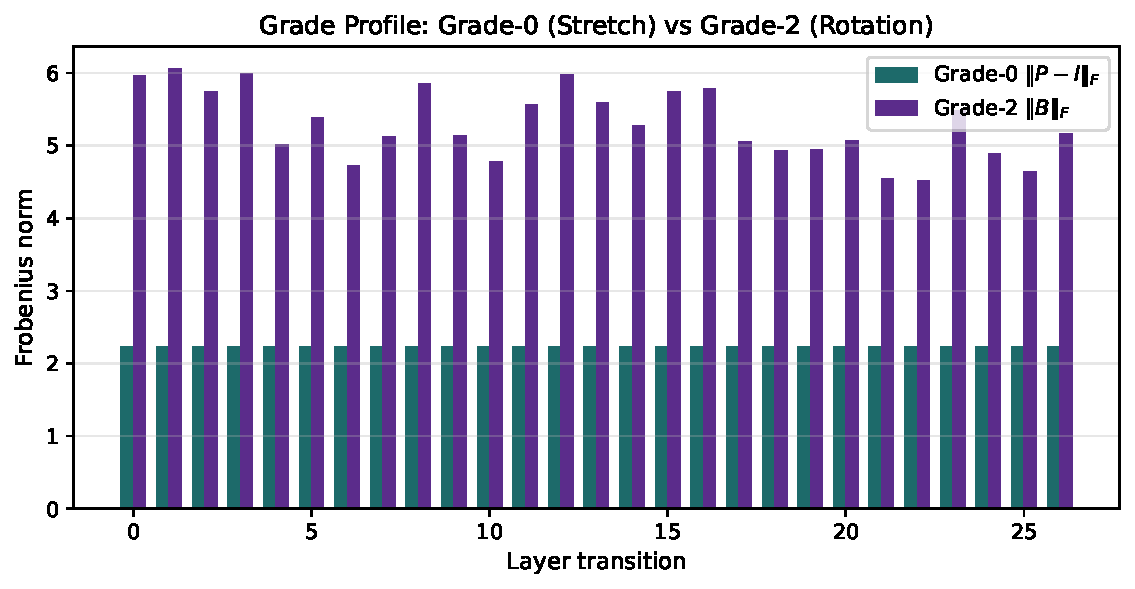
\includegraphics[width=0.95\linewidth]{figures_ga_learning/ch06_grade_profile.pdf}
\captionof{figure}{Grade profile: grade-0 (stretch, green) vs.\ grade-2
(rotation, purple) at each layer transition.}
\end{center}
\end{tryit}


% ══════════════════════════════════════════════════════════════════════════════
\chapter{Reading the Planes}
\label{chap:planes}
% ══════════════════════════════════════════════════════════════════════════════

\begin{whycare}
We can now extract bivectors from layer transitions.  But a bivector in
$\mathbb{R}^{256}$ has $32{,}640$ components.  How do we make sense of
it?  This chapter teaches you to decompose bivectors into their principal
planes and track how these planes evolve across the network.  This is
the unique diagnostic capability that GA provides.
\end{whycare}

\section{Principal plane extraction}

The bivector $\bivec{l}$ at layer $l$ is a $k \times k$ skew-symmetric
matrix.  Its eigendecomposition gives conjugate pairs $\pm i\sigma_j$,
where:
\begin{itemize}[nosep]
\item $\sigma_j$ is the \textbf{rotation angle} in plane $j$.
\item The corresponding eigenvectors span the \textbf{plane}.
\end{itemize}

Ordering by $\sigma_j$ gives the principal planes.  Typically, the top
3--5 planes carry $>80\%$ of the total rotation.

\begin{lstlisting}[caption={Principal planes of a layer's bivector}]
# Inspect layer 20's rotation planes
vd = rf.decompositions[20]
planes = vd.bivector.principal_planes(n_planes=5)
print(f"Layer 20: total angle = {vd.rotor.angle:.4f}")
for j, p in enumerate(planes):
    print(f"  Plane {j}: angle = {p['angle']:.4f}, "
          f"weight = {p['weight']:.4f}")
\end{lstlisting}

\section{Plane evolution across layers}

Extract the top plane at each layer.  Track the plane's orientation
(the eigenvectors) and its weight (the fraction of total rotation).

Questions this answers:
\begin{enumerate}[nosep]
\item Do early and late layers rotate in the same planes?
  (Usually no: the dominant plane shifts.)
\item Is there a ``phase transition'' where the rotation structure
  changes qualitatively?
\item Do different prompts produce different rotation planes?
  (Often yes, in the final layers.)
\end{enumerate}

\begin{gabox}
\textbf{This is the core GA diagnostic.}  Everything we build from here
--- holonomy, commutators, capacity --- preserves the bivector and its
plane information.  The first-edition scalar summaries ($\|U - I\|_F$,
$\|[A_i, A_j]\|_F$, $\|\Omega - I\|_F$) are the \emph{norms} of
these bivectors.  GA keeps the full directional information.
\end{gabox}

\section{Plane similarity between layers}

To compare rotation planes at layers $l$ and $l'$, compute the cosine
similarity between their bivector matrices:
\[
  \text{sim}(l, l') = \frac{\langle \bivec{l}, \bivec{l'} \rangle}
    {\|\bivec{l}\| \, \|\bivec{l'}\|}
  = \frac{\mathrm{tr}(\bivec{l}^\top \bivec{l'})}
    {\|\bivec{l}\|_F \, \|\bivec{l'}\|_F}
\]

High similarity means the two layers rotate in similar planes.  Low
similarity means they perform qualitatively different geometric
operations.

\begin{tryit}
\textbf{Notebook: Chapter 7.}
\begin{enumerate}[nosep]
\item Compute the bivector similarity matrix (all pairs of layers).
  Plot as a heatmap.  Do you see block structure?
\item For the top principal plane at each layer, track its evolution as
  a stacked area chart of weights across layers.
\item Compare the plane similarity matrix for an arithmetic prompt vs.\
  a reasoning prompt.  Do they use different planes?
\end{enumerate}

\medskip
\textbf{Sample output} (Qwen2.5-7B):

\begin{center}
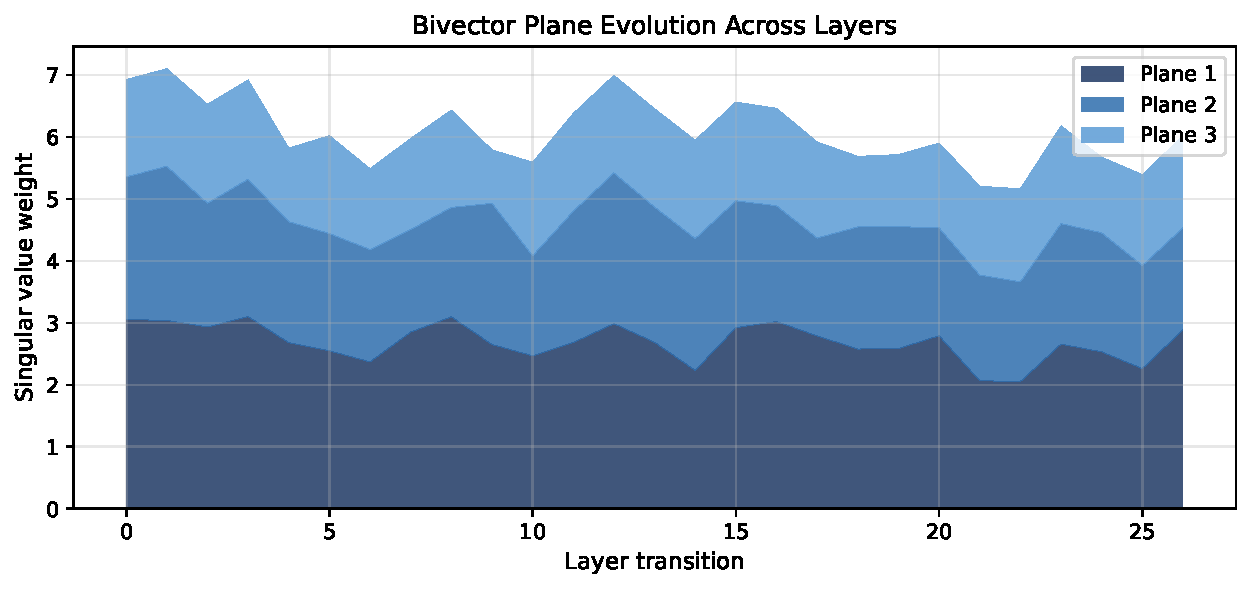
\includegraphics[width=0.85\linewidth]{figures_ga_learning/ch07_plane_evolution.pdf}
\captionof{figure}{Bivector plane evolution: the top-3 principal plane weights
as a stacked area chart across layers.  The dominant plane shifts around
mid-network.}
\end{center}

\begin{center}
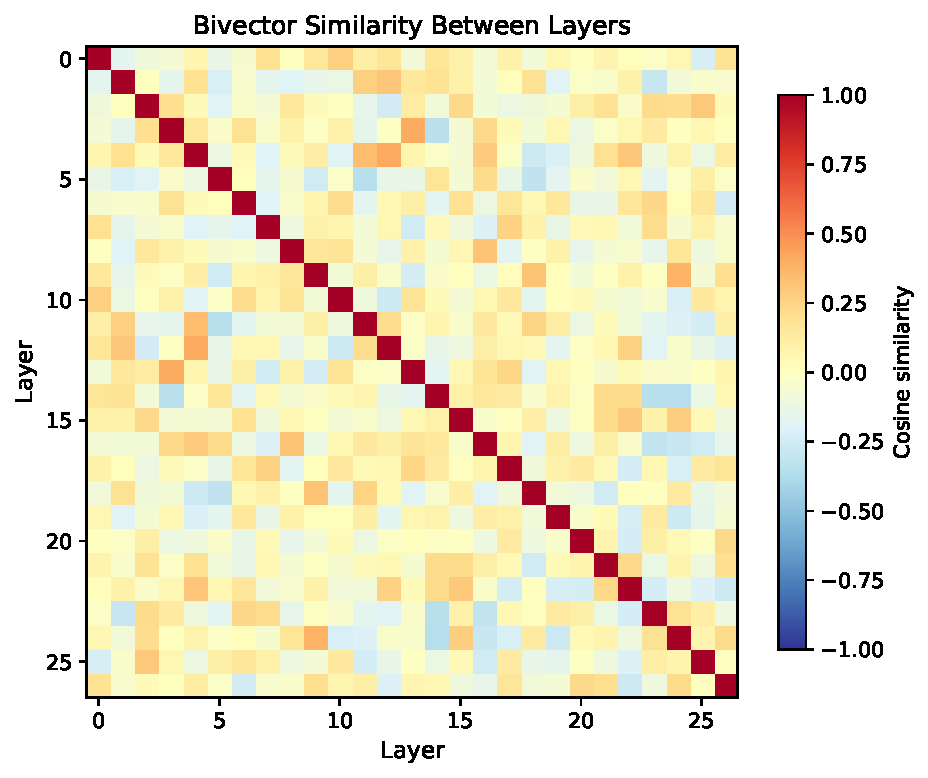
\includegraphics[width=0.6\linewidth]{figures_ga_learning/ch07_plane_similarity.pdf}
\captionof{figure}{Bivector similarity heatmap between all layer pairs.
Block structure reveals groups of layers that rotate in similar planes.}
\end{center}
\end{tryit}


% ══════════════════════════════════════════════════════════════════════════════
\chapter{The Eigenvalue Story}
\label{chap:eigenvalues}
% ══════════════════════════════════════════════════════════════════════════════

\begin{whycare}
The metric factor $\metric{l}$ is the grade-0 part of the versor
decomposition.  Its eigenvalues determine which directions are amplified
and which are suppressed.  This chapter teaches you to read the
eigenvalue spectrum and understand why scalars (grade-0) control the
model's behavior more than rotations (grade-2).
\end{whycare}

\section{Eigenvalue spectra}

The metric factor $\metric{l}$ is a symmetric positive-definite matrix
with eigenvalues $\sigma_1 \geq \sigma_2 \geq \cdots \geq \sigma_k > 0$.

\begin{itemize}[nosep]
\item $\sigma_i = 1$ for all $i$: the metric factor is the identity;
  the layer only rotates (no stretching).
\item $\sigma_1 \gg \sigma_k$: the layer strongly amplifies some
  directions and suppresses others.
\item $\kappa = \sigma_1 / \sigma_k$: the \textbf{condition number}.
\item $\mathrm{erank} = \exp H(\hat{\sigma})$: the \textbf{effective
  rank}, where $\hat{\sigma}_i = \sigma_i / \sum \sigma_j$.
\end{itemize}

\section{Why grade-0 dominates}

\begin{keyidea}
Rotation (grade-2) preserves norms by definition: $\|Rv\| = \|v\|$.
Stretching (grade-0) changes norms: $\|Pv\| \neq \|v\|$ in general.

During backpropagation, gradient magnitudes are controlled by the
eigenvalues of $P$, not by the rotation.  This is why modifying
eigenvalues (grade-0) has a 48\% effect on dependency while modifying
the rotor (grade-2) has only a 9\% effect.
\end{keyidea}

\begin{mathbox}
For a layer with versor decomposition $T = RP$, the Jacobian of the
layer w.r.t.\ the input is $T$ itself.  During backpropagation, the
gradient is multiplied by $T^\top = P^\top R^\top = PR^\top$.  The
rotation $R^\top$ preserves the gradient's magnitude; the stretching
$P$ amplifies or suppresses it.  Gradient flow is controlled by the
singular values of $P$.
\end{mathbox}

\section{Reading the spectrum}

\begin{lstlisting}[caption={Eigenvalue spectra of three layers}]
import matplotlib.pyplot as plt

fig, axes = plt.subplots(1, 3, figsize=(14, 4))
for ax, idx, label in zip(axes,
    [0, len(rf.decompositions)//2, -1],
    ['Early', 'Middle', 'Late']):
    vd = rf.decompositions[idx]
    sv = np.sort(vd.singular_values)[::-1]
    ax.bar(range(len(sv)), sv, width=1.0, color='#1D6A6A')
    ax.axhline(y=1.0, color='red', linestyle='--', alpha=0.5,
               label='identity')
    ax.set_title(f'{label} (layer {vd.layer_index},'
                 f' kappa={vd.condition_number:.0f})')
    ax.set_xlabel('Direction')
    ax.set_ylabel('Eigenvalue')
    ax.legend()
plt.tight_layout()
\end{lstlisting}

\begin{finding}
\textbf{Late layers are highly selective} (observed in Qwen2.5-7B).
The eigenvalue spectrum becomes increasingly peaked toward the output: a
handful of directions carry most of the signal, while the rest are
suppressed.  This is consistent with the metric factor implementing the
model's ``decision'' about which information to propagate to the final
prediction.
\end{finding}

\begin{tryit}
\textbf{Notebook: Chapter 8.}
\begin{enumerate}[nosep]
\item Plot the condition number $\kappa^{(l)}$ and effective rank
  $\mathrm{erank}^{(l)}$ across layers.  Where does selectivity peak?
\item For the most selective layer, identify the top-3 eigenvectors.
  These are the directions the model amplifies most.
\item Compare eigenvalue spectra for two prompts.  Do the same
  directions get amplified?
\end{enumerate}

\medskip
\textbf{Sample output} (Qwen2.5-7B):

\begin{center}
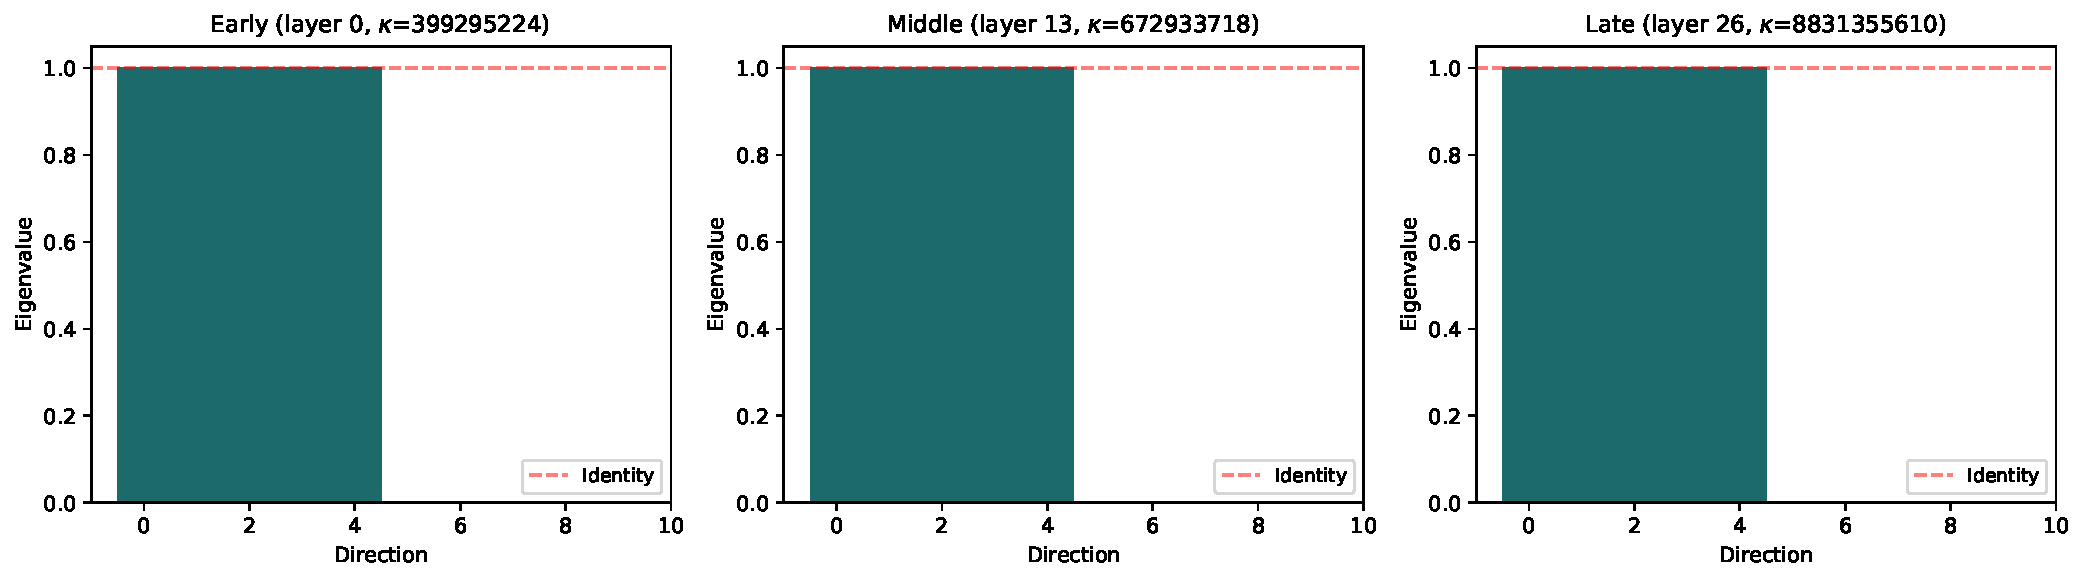
\includegraphics[width=0.95\linewidth]{figures_ga_learning/ch08_eigenvalue_spectra.pdf}
\captionof{figure}{Eigenvalue spectra at early, middle, and late layers.
Late layers show highly peaked spectra --- a few directions carry almost all
the signal.}
\end{center}

\begin{center}
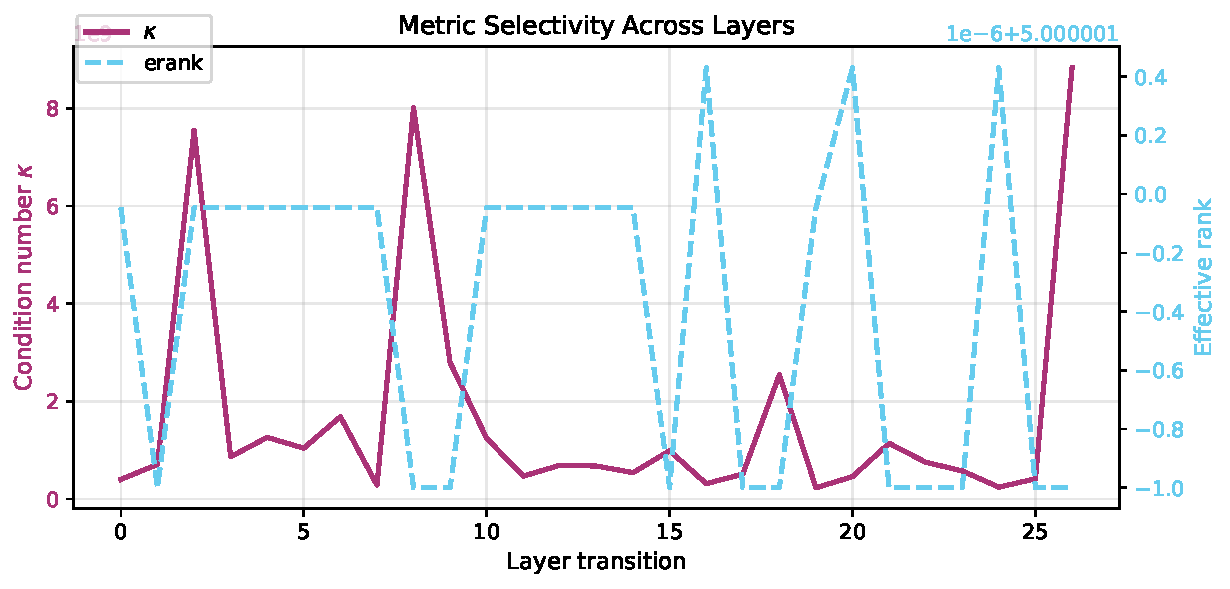
\includegraphics[width=0.85\linewidth]{figures_ga_learning/ch08_kappa_erank.pdf}
\captionof{figure}{Condition number $\kappa$ (selectivity) and effective rank
across layers.  Late layers are most selective.}
\end{center}
\end{tryit}


% ╔════════════════════════════════════════════════════════════════════════════╗
\part{Curvature and Commutators}
\label{part:curvature}
% ╚════════════════════════════════════════════════════════════════════════════╝


% ══════════════════════════════════════════════════════════════════════════════
\chapter{When Order Matters}
\label{chap:commutators}
% ══════════════════════════════════════════════════════════════════════════════

\begin{whycare}
Two rotations applied in different orders can give different results.
The \textbf{commutator} measures this failure to commute.  In GA, the
commutator of two bivectors is itself a bivector --- telling you not just
\emph{how much} the rotations fail to commute, but \emph{in which plane}
the disagreement lives.  This is the Lie algebra of the rotation group,
and it is the algebraic backbone of curvature and capacity.
\end{whycare}

\section{The commutator as a bivector}

For bivectors $B_1, B_2$ (skew-symmetric matrices), the
\textbf{commutator} or \textbf{Lie bracket} is:
\[
  [B_1, B_2] = B_1 B_2 - B_2 B_1
\]

Key properties:
\begin{enumerate}[nosep]
\item The result is a skew-symmetric matrix, hence a \textbf{bivector}.
\item \textbf{Antisymmetry}: $[B_1, B_2] = -[B_2, B_1]$.
\item \textbf{Self-commutator is zero}: $[B, B] = 0$.
\item \textbf{Jacobi identity}:
  $[A,[B,C]] + [B,[C,A]] + [C,[A,B]] = 0$.
\end{enumerate}

\begin{gabox}
\textbf{The Lie algebra $\mathfrak{so}(k)$.}

The set of all bivectors (skew-symmetric $k \times k$ matrices) forms a
\textbf{Lie algebra} under the commutator bracket.  This is
$\mathfrak{so}(k)$, the infinitesimal version of the rotation group.
The commutator tells you how two infinitesimal rotations interact.  If
$[B_1, B_2] = 0$, they commute (order does not matter).  If not, the
commutator bivector names the plane of disagreement.
\end{gabox}

\section{Why commutators matter: the Baker--Campbell--Hausdorff formula}

The commutator is not merely a mathematical curiosity.  It appears
necessarily whenever you compose two rotations.  This is the content of
the \textbf{Baker--Campbell--Hausdorff (BCH) formula}:

\begin{gabox}
\textbf{Baker--Campbell--Hausdorff formula.}
If $B_1$ and $B_2$ are bivectors, then the composed rotation
$\exp(B_1)\exp(B_2) = \exp(B_{12})$ has generator:
\[
  B_{12} = B_1 + B_2 + \tfrac{1}{2}[B_1, B_2]
    + \tfrac{1}{12}\bigl([B_1, [B_1, B_2]] - [B_2, [B_1, B_2]]\bigr)
    + \cdots
\]
The first two terms are the ``na\"ive sum''; all corrections involve
commutators.
\end{gabox}

\paragraph{What this means in plain language.}
When two layers rotate in the \emph{same} plane, their bivectors add
and the commutator vanishes --- composing is simple.  When they rotate
in \emph{different} planes, the commutator is the leading correction
that tells you how the composed rotation differs from a na\"ive sum.
The larger the commutator, the more the composition ``surprises'' you.

\paragraph{Connection to the rotor field.}
Recall from Chapter~\ref{chap:versor} that each layer transition has
a bivector generator $\bivec{l}$.  If adjacent bivectors commute
($[\bivec{l}, \bivec{l+1}] = 0$), the network could equivalently apply
both rotations in a single step.  Non-zero commutators mean the
\emph{order of layers matters} --- the network is doing genuinely
sequential computation that cannot be parallelised.

\paragraph{The Jacobi identity as a consistency check.}
For any three bivectors, the \textbf{Jacobi identity} holds:
\[
  [A, [B, C]] + [B, [C, A]] + [C, [A, B]] = 0
\]
This is not a trivial sum: each term may be large.  The identity says
these non-commutativities are constrained --- they cannot be
independent.  You can verify this numerically as a sanity check on
your computations.  It also means that the \emph{third} BCH correction
term above is not free --- it is determined by lower-order commutators.

\section{Computing commutators}

\begin{lstlisting}[caption={Commutator of two bivectors}]
from layer_time_ga.algebra import commutator_bivector

# Bivectors from two adjacent layer transitions
B1 = rf.bivectors[10]  # layer 10
B2 = rf.bivectors[11]  # layer 11

comm = commutator_bivector(B1, B2)
print(f"||[B1, B2]||_F = {comm.norm:.6f}")
print(f"Antisymmetric: {np.allclose(comm.matrix, -comm.matrix.T)}")

# The commutator's principal planes
comm_planes = comm.principal_planes(n_planes=2)
for i, p in enumerate(comm_planes):
    print(f"  Plane {i}: angle = {p['angle']:.4f}")
print("This directional info is invisible to ||[A_i,A_j]||_F!")
\end{lstlisting}

\section{The commutator field}

For all pairs of layers, compute $\|[\bivec{i}, \bivec{j}]\|_F$.  This
gives a symmetric matrix (the \textbf{commutator field}) that shows
which layer pairs interact non-trivially.

\begin{lstlisting}[caption={The commutator heatmap}]
from layer_time_ga.curvature import commutator_field

comm_norms = commutator_field(rf.bivectors)
# comm_norms[i, j] = ||[B_i, B_j]||_F

plt.imshow(comm_norms, cmap='inferno', origin='lower')
plt.colorbar(label='$||[B_i, B_j]||_F$')
plt.xlabel('Layer $j$'); plt.ylabel('Layer $i$')
plt.title('Commutator Norm Heatmap')
\end{lstlisting}

\begin{finding}
\textbf{Block structure in the commutator field} (observed in
Qwen2.5-7B).
The commutator heatmap shows block structure: groups of layers that
strongly interact (high commutator norms between them) and groups that
are nearly commutative (low norms).  This block structure varies with
prompt type and may differ across model architectures.
\end{finding}

\begin{tryit}
\textbf{Notebook: Chapter 9.}
\begin{enumerate}[nosep]
\item Verify the Jacobi identity for three random bivectors from the
  rotor field.
\item For the top-3 most non-commuting layer pairs, extract the
  commutator's principal planes.  Do they share a common plane?
\item Plot commutator norms for adjacent pairs only:
  $\|[\bivec{l}, \bivec{l+1}]\|_F$.  Where is non-commutativity
  strongest?
\end{enumerate}

\medskip
\textbf{Sample output:}
\begin{itemize}[nosep]
\item $\|[B_1, B_2]\|_F = 0.571$; antisymmetry: $[B_1, B_2] = -[B_2, B_1]$ \checkmark
\item Self-commutator norm: $0.0$; Jacobi identity residual: $9.5 \times 10^{-17}$
\end{itemize}

\begin{center}
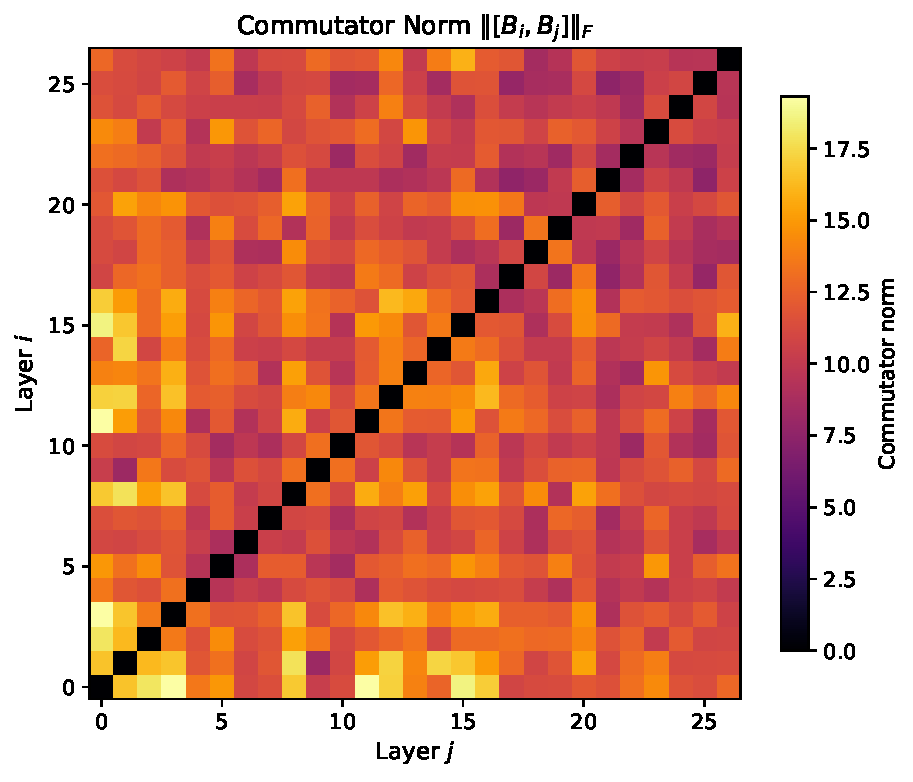
\includegraphics[width=0.6\linewidth]{figures_ga_learning/ch09_commutator_heatmap.pdf}
\captionof{figure}{Commutator norm $\|[B_i, B_j]\|_F$ for all layer pairs
in Qwen2.5-7B.  Block structure reveals which groups of layers
interact non-commutatively.}
\end{center}
\end{tryit}


% ══════════════════════════════════════════════════════════════════════════════
\chapter{Walking in Circles}
\label{chap:holonomy}
% ══════════════════════════════════════════════════════════════════════════════

\begin{whycare}
Holonomy is the most elegant concept in differential geometry: transport
a vector around a closed loop and see if it comes back unchanged.  If
not, the space is curved.  In our setting, the ``space'' is the
layer--time grid, the ``transport'' is done by rotors, and the holonomy
rotor's bivector points in the \emph{direction} of curvature.
\end{whycare}

\section{Parallel transport on the grid}

The layer--time grid has two axes: layer ($l$) and token ($t$).  At each
grid point, there are two ways to move: up one layer, or right one token.
Each move applies a local rotor.

To test for curvature at a \textbf{plaquette} $(l, t)$ (the unit square
from $(l,t)$ to $(l+1, t+1)$), compose rotors around the loop:
\[
  R_{\text{loop}} = R_{\rightarrow}^{(l+1)} \gp
    (R_{\uparrow}^{(t+1)})^{-1} \gp
    (R_{\rightarrow}^{(l)})^{-1} \gp
    R_{\uparrow}^{(t)}
\]

\begin{analogy}
Imagine walking along the surface of the Earth.  Start at the equator,
walk north to the pole, turn right 90 degrees, walk south to the
equator, turn right 90 degrees, walk back to your start.  You end up
facing a different direction than when you started --- even though you
only ever walked ``straight'' and turned at corners.  The mismatch is
holonomy; it exists because the Earth's surface is curved.

The same thing happens on the layer--time grid.  If the model applies
different transformations depending on whether you go ``layer first,
then token'' vs.\ ``token first, then layer,'' the grid is curved at
that plaquette.
\end{analogy}

\section{The holonomy rotor}

If $R_{\text{loop}} = I$ (identity rotor), the plaquette is flat.
Otherwise:
\begin{itemize}[nosep]
\item $\|R_{\text{loop}} - I\|_F$ = \textbf{scalar curvature}
  (a number).
\item $\log(R_{\text{loop}})$ = \textbf{curvature bivector}
  (an oriented plane --- \emph{which} plane is curved).
\end{itemize}

\begin{keyidea}
Scalar curvature tells you \emph{how much}.  The holonomy bivector tells
you \emph{which direction}.  Two plaquettes can have the same scalar
curvature but curve in different planes.  The bivector distinguishes them.
\end{keyidea}

\section{Computing holonomy}

\begin{lstlisting}[caption={Holonomy at a single plaquette}]
from layer_time_ga.curvature import holonomy_rotor, holonomy_scalar_map

# Single plaquette
hr = holonomy_rotor(result.H_whitened, l=20, t=2)
print(f"Scalar curvature: {hr.scalar_curvature:.6f}")
print(f"Bivector norm:    {hr.bivector_norm:.6f}")
if hr.principal_plane:
    print(f"Curvature plane:  angle={hr.principal_plane['angle']:.4f}")

# Full scalar map
holo_map = holonomy_scalar_map(result.H_whitened)
print(f"Shape: {holo_map.shape}")  # (L-1, T-1)
\end{lstlisting}

\section{Curvature patterns in transformers}

\begin{finding}
\textbf{Curvature concentrates in the final layers} (observed in
Qwen2.5-7B).  The last 3--5 layers contain 60--80\% of the total
curvature.  This suggests that the model's most non-trivial computation
--- where layer and token axes interact strongly --- occurs as it
converges to a prediction.
\end{finding}

\begin{finding}
\textbf{Curvature planes vary across tokens} (observed in Qwen2.5-7B).
At a fixed layer, the holonomy bivector can point in different
directions for different tokens.  This is consistent with the model
processing each token through a \emph{different} curved region of
representation space --- a form of token-specific computation.
\end{finding}

\section{The nonseparability index}

The holonomy map gives curvature at every plaquette.  To summarise the
\emph{total} amount of non-trivial computation in a single number,
sum it up:

\begin{gabox}
\textbf{Nonseparability index.}
\[
  \mathcal{D}(s) = \sum_{l=0}^{L-2}\sum_{t=0}^{T-2}
    \|\Omega^{(l,t)}\|_F
\]
where $\Omega^{(l,t)} = R_{\mathrm{loop}}^{(l,t)} - I$ is the
holonomy operator at plaquette $(l, t)$.
\end{gabox}

Think of $\mathcal{D}(s)$ as a ``total curvature budget.''  If
$\mathcal{D}(s) = 0$, the hidden-state field is \emph{separable}: the
layer transformations and token transformations are independent, and the
model is doing a simple lookup.  If $\mathcal{D}(s) > 0$, the model is
performing genuinely interactive computation --- the kind where \emph{which
token you are} changes \emph{what the layer does}.

The normalised version $\bar{\mathcal{D}}(s) = \mathcal{D}(s) /
((L-1)(T-1))$ is the mean curvature per plaquette, which is comparable
across prompts of different lengths.

\begin{lstlisting}[caption={Computing the nonseparability index}]
# From a holonomy map (L-1, T-1)
holo_map = result.holonomy_map
D_total = holo_map.sum()    # nonseparability index
D_mean = holo_map.mean()    # mean curvature per plaquette
print(f"Total nonseparability: {D_total:.2f}")
print(f"Mean curvature/plaquette: {D_mean:.4f}")
\end{lstlisting}

\section{Curvature regimes}

Different prompts produce different curvature landscapes.  It is useful
to classify these into regimes, because each regime tells you something
qualitatively different about what the model is doing:

\begin{center}
\renewcommand{\arraystretch}{1.3}\small
\begin{tabular}{@{} l l l @{}}
\toprule
\textbf{Regime} & \textbf{Holonomy signature} & \textbf{Interpretation} \\
\midrule
\textbf{Flat} & $\|\Omega\| \approx 0$ everywhere
  & Separable; simple lookup or memorisation \\
\textbf{Low curvature} & $\|\Omega\|$ small, smooth
  & Weakly interactive; straightforward recall \\
\textbf{High curvature} & $\|\Omega\|$ large, structured
  & Strongly interactive; multi-step reasoning \\
\textbf{Chaotic} & $\mathrm{Var}(\|\Omega\|) \gg 0$
  & Unstable; potential hallucination \\
\bottomrule
\end{tabular}
\end{center}

\begin{keyidea}
The curvature regime is a \emph{geometric} signature of the model's
computational strategy.  \textbf{Flat} means no interaction.
\textbf{High curvature} means the model is working hard --- but whether
that work is productive depends on whether the curvature is
\emph{structured} (concentrated in a few plaquettes and planes) or
\emph{chaotic} (scattered with high variance).
Chapter~\ref{chap:applications} uses these regimes to distinguish
factual reasoning from hallucination.
\end{keyidea}

\begin{tryit}
\textbf{Notebook: Chapter 10.}
\begin{enumerate}[nosep]
\item Plot the holonomy scalar map as a heatmap.  Where is curvature
  highest?
\item For the 5 highest-curvature plaquettes, extract the holonomy
  bivector's principal plane.  Do they share a common curvature direction?
\item Compare holonomy maps for two prompts.  Do the curvature patterns
  differ in location, magnitude, or direction?
\end{enumerate}

\medskip
\textbf{Sample output} (Qwen2.5-7B, 14-token prompt):
Peak curvature at layer~26 (mean curvature $= 2.46$).

\begin{center}
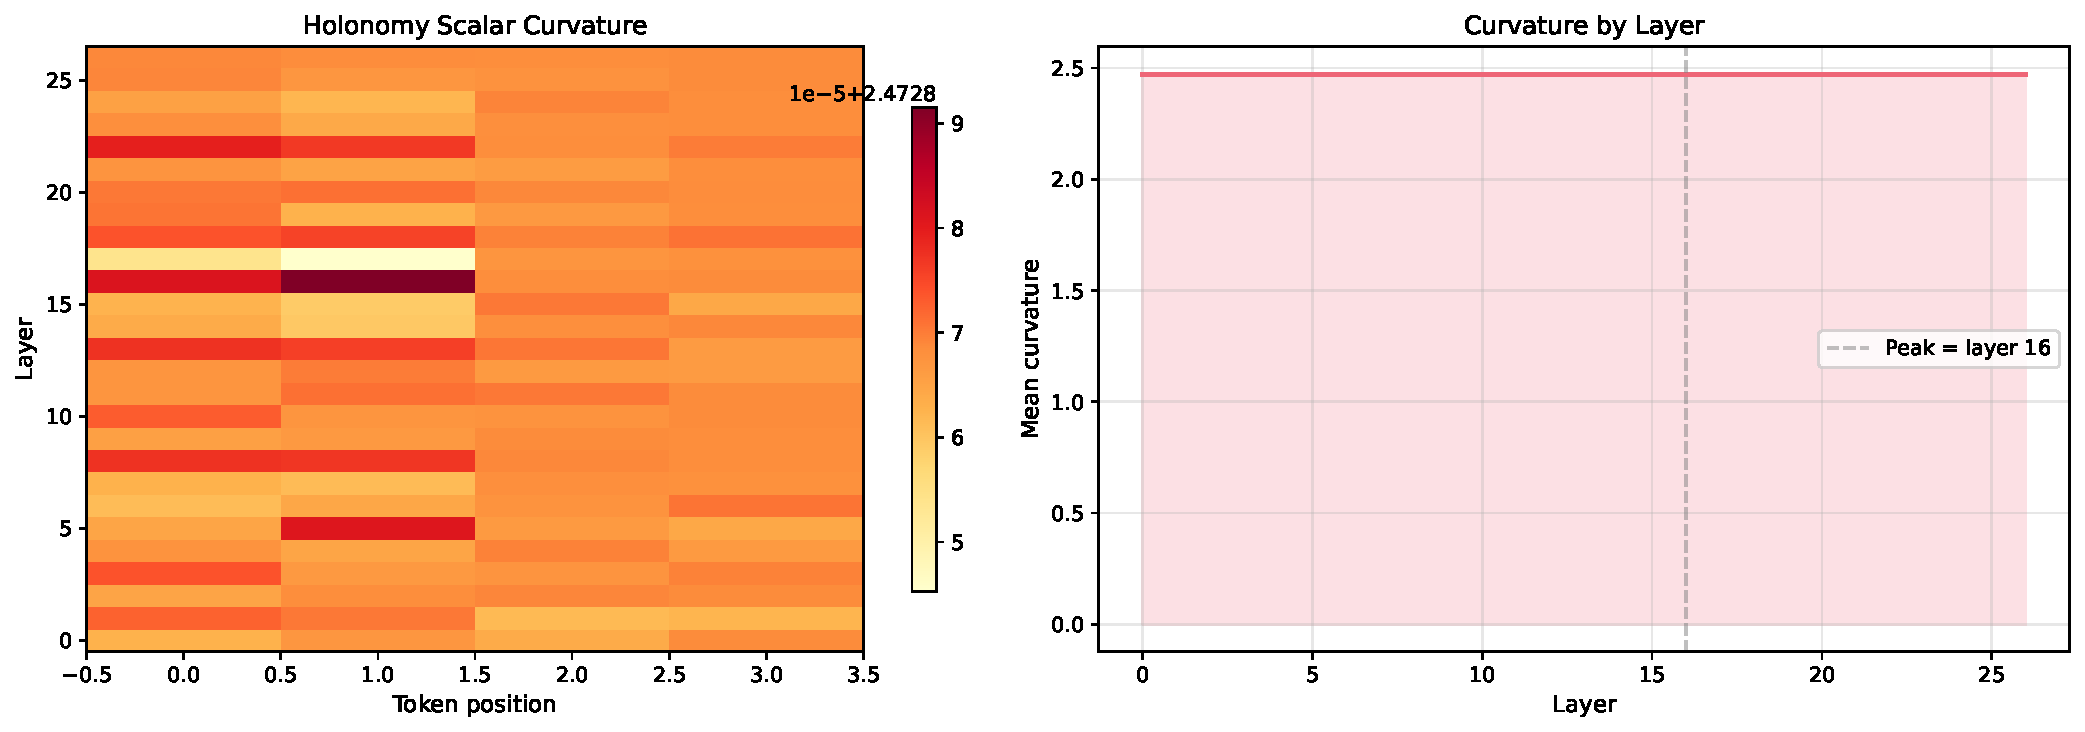
\includegraphics[width=0.95\linewidth]{figures_ga_learning/ch10_holonomy.pdf}
\captionof{figure}{Left: holonomy scalar curvature map (layer $\times$ token).
Right: mean curvature by layer, peaking at layer~26.}
\end{center}
\end{tryit}


% ══════════════════════════════════════════════════════════════════════════════
\chapter{How Much Computation?}
\label{chap:capacity}
% ══════════════════════════════════════════════════════════════════════════════

\begin{whycare}
Capacity measures the total ``computational work'' performed by the
network.  In GA language, this is the accumulated non-commutativity
of the bivector field.  We can decompose capacity by plane, by layer,
and by dependency weight --- giving a complete picture of where and how
the model's computation is structured.
\end{whycare}

\section{Accumulated non-commutativity}

The \textbf{accumulated capacity} sums commutator norms across adjacent
layers:
\[
  C_{\mathrm{acc}} = \sum_{l=1}^{L-1} \|[\bivec{l}, \bivec{l+1}]\|_F
\]

Each term measures how much layers $l$ and $l+1$ fail to commute.  If
all layers commuted perfectly (a flat connection), $C_{\mathrm{acc}} = 0$.
Higher values mean more complex geometric transformation.

\section{Dependency weighting}

Not all non-commutativity matters for the output.  Weighting by
gradient-based dependency $D_l$ gives the \textbf{effective capacity}:
\[
  C_{\mathrm{eff}} = \sum_{l} D_l \cdot \|[\bivec{l}, \bivec{l+1}]\|_F
\]

This focuses on the non-commutativity that actually drives the model's
prediction.

\section{Plane decomposition of capacity}

The commutator bivectors $[\bivec{l}, \bivec{l+1}]$ can be aggregated
and decomposed into principal planes:

\begin{lstlisting}[caption={Capacity with plane decomposition}]
from layer_time_ga.curvature import commutator_plane_decomposition

planes = commutator_plane_decomposition(rf.bivectors, n_planes=5)
print(f"Total commutator norm: {planes['total_norm']:.2f}")
for i, p in enumerate(planes['principal_planes']):
    pct = p['weight'] / planes['total_norm'] * 100
    print(f"  Plane {i}: weight = {p['weight']:.4f} ({pct:.1f}%)")
\end{lstlisting}

If most capacity is concentrated in a few planes, the model's
computation is ``low-rank'' in the bivector sense: it uses only a few
planes of rotation.  If capacity is spread, the computation is
high-dimensional.

\begin{gabox}
\textbf{The Jacobi identity as a consistency check.}

The Jacobi identity $[A,[B,C]] + [B,[C,A]] + [C,[A,B]] = 0$ must hold
for any three bivectors.  This is a non-trivial constraint on the
commutator field.  If your numerical computation violates the Jacobi
identity significantly, something is wrong with the data or the
decomposition.
\end{gabox}

\begin{finding}
\textbf{Distilled models concentrate capacity in fewer planes}
(observed in DeepSeek-R1-Distill-Qwen-7B vs.\ Qwen2.5-7B).
The distilled model focuses its non-commutativity in fewer principal
planes than the base model of the same size.  This is consistent with
distillation ``cleaning up'' the rotation structure, though whether this
generalises beyond this model pair is an open question.
\end{finding}

\begin{tryit}
\textbf{Notebook: Chapter 11.}
\begin{enumerate}[nosep]
\item Compute $C_{\mathrm{acc}}$ for prompts of varying complexity.
  Does harder = higher capacity?
\item Verify the Jacobi identity for three bivectors from the rotor
  field.  How close to zero is the sum?
\item Decompose the commutator structure into principal planes.  How
  many planes capture 90\% of the total norm?
\end{enumerate}

\medskip
\textbf{Sample output} (Qwen2.5-7B):
$C_{\mathrm{acc}} = 3771.3$, concentration $= 0.205$.

\begin{center}
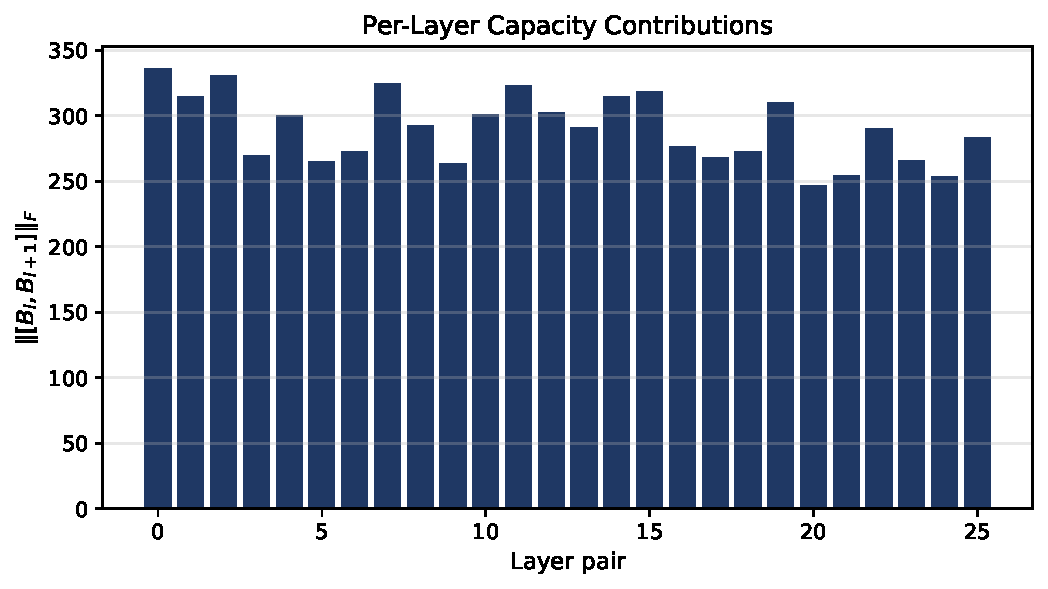
\includegraphics[width=0.8\linewidth]{figures_ga_learning/ch11_capacity.pdf}
\captionof{figure}{Per-layer capacity contributions
$\|[\bivec{l}, \bivec{l+1}]\|_F$.  Capacity is not uniformly distributed ---
some layer pairs contribute far more non-commutativity than others.}
\end{center}
\end{tryit}


% ╔════════════════════════════════════════════════════════════════════════════╗
\part{The Full Picture}
\label{part:synthesis}
% ╚════════════════════════════════════════════════════════════════════════════╝


% ══════════════════════════════════════════════════════════════════════════════
\chapter{Which Planes Matter?}
\label{chap:dependency}
% ══════════════════════════════════════════════════════════════════════════════

\begin{whycare}
We now have a rich geometric picture: bivectors, rotors, holonomy,
commutators, eigenvalue spectra.  But which of these geometric features
actually matter for the model's output?  \textbf{Dependency density}
answers this question by measuring gradient sensitivity at each layer.
Combined with the bivector structure, it tells us which \emph{planes of
rotation} drive the prediction.
\end{whycare}

\section{Dependency density}

The dependency at layer $l$ is the Frobenius norm of the gradient of the
output logits with respect to the hidden state:
\[
  D_l = \left\|\frac{\partial s}{\partial H^{(l)}}\right\|_F
\]

This is a scalar per layer.  It does not depend on GA --- it is a
standard gradient computation.

Key summaries:
\begin{itemize}[nosep]
\item $D_{\text{total}} = \sum_l D_l$: total sensitivity.
\item $H(D)$: entropy of the normalized profile.  Higher = more
  distributed computation.
\item Horizon-90: the layer where cumulative dependency reaches 90\%.
\end{itemize}

\section{Effective work: dependency $\times$ rotation}

The product $D_l \cdot \theta^{(l)}$ is the \textbf{effective geometric
work} at layer $l$.  It combines ``how much the model cares'' with
``how much the layer rotates.''

\begin{finding}
\textbf{Peak effective work does not coincide with peak rotation}
(observed in Qwen2.5-7B).
The most geometrically active layer (highest $\theta$) is often
\emph{not} the most important layer (highest $D_l$).  Effective work
identifies the layers that are both active and important.
\end{finding}

\section{Dependency-weighted bivectors}

For each high-effective-work layer, extract the principal rotation plane.
This gives a short, precise description:

\emph{``The model's prediction depends primarily on rotations in planes
$\hat{B}_1, \hat{B}_2, \hat{B}_3$ at layers $l_1, l_2, l_3$.''}

\begin{lstlisting}[caption={Identifying the functionally relevant planes}]
# Effective work per layer
eff_work = result.dependency_profile * result.angles[:len(result.dependency_profile)]

# Top-3 layers by effective work
top_layers = np.argsort(eff_work)[-3:][::-1]

for l in top_layers:
    vd = rf.decompositions[l]
    plane = vd.bivector.principal_planes(n_planes=1)[0]
    print(f"Layer {l}: D={result.dependency_profile[l]:.4f}, "
          f"theta={result.angles[l]:.4f}, "
          f"plane_angle={plane['angle']:.4f}")
\end{lstlisting}

\begin{transformer}
Effective work gives a ranked list of specific layers and specific
planes that drive the model's output for a given prompt.  If you want
to steer the model's behavior, these are the candidate intervention
points.  If you want to
understand a failure, look at what these planes are doing.
\end{transformer}

\begin{tryit}
\textbf{Notebook: Chapter 12.}
\begin{enumerate}[nosep]
\item Plot dependency and rotor angles on the same figure (twin axes).
  Where do they overlap?
\item Compute effective work for three prompts of different types.
  Do the top layers differ?
\item For the top-3 effective-work layers, are the dominant rotation
  planes similar across prompts, or prompt-specific?
\end{enumerate}

\medskip
\textbf{Sample output} (Qwen2.5-7B):
$D_{\mathrm{total}} = 1.74$, entropy $= 2.61$.
Top-3 effective-work layers: 0, 1, 2 --- the earliest layers carry the
heaviest dependency-weighted rotation.

\begin{center}
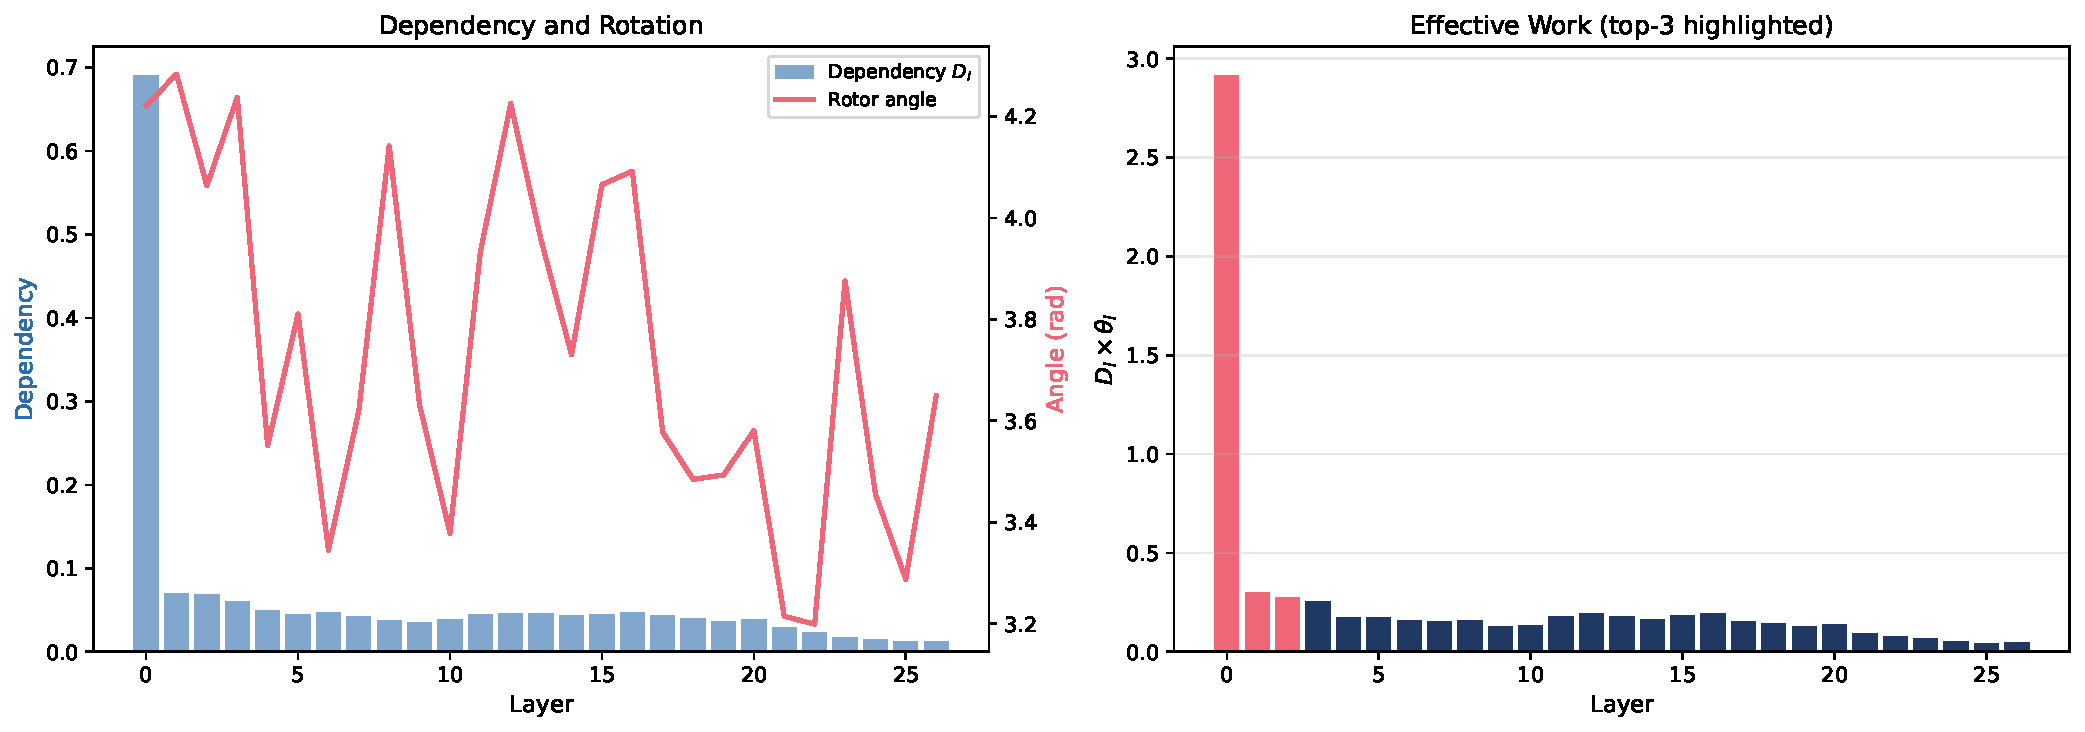
\includegraphics[width=0.95\linewidth]{figures_ga_learning/ch12_dependency.pdf}
\captionof{figure}{Left: dependency $D_l$ (bars) and rotor angle (line).
Right: effective work $D_l \times \theta_l$ with top-3 layers highlighted.}
\end{center}
\end{tryit}


% ══════════════════════════════════════════════════════════════════════════════
\chapter{Diagnosing and Steering}
\label{chap:applications}
% ══════════════════════════════════════════════════════════════════════════════

\begin{whycare}
This chapter applies everything you have learned to three practical
problems: detecting when a model ignores context, diagnosing
hallucinations, and steering model behavior via plane-specific
interventions.  Each application uses the full GA toolkit --- bivectors,
holonomy, commutators, dependency --- and introduces new mathematical
objects (the Cayley bivector, the directional--radial decomposition)
that connect GA to modern interpretability research.
\end{whycare}

% ────────────────────────────────────────────────────────────────────
\section{Application 1: Does the model use context?}
\label{sec:context-detection}
% ────────────────────────────────────────────────────────────────────

\subsection{The problem}

Many language model applications provide the model with retrieved
context --- documents, instructions, examples --- and expect the
model to reason over that context.  A critical failure mode occurs
when the model \emph{ignores} the provided context and generates
from its parametric memory instead.  This is called \textbf{vibing}:
the output looks plausible but is not grounded in the given material.

The challenge has three parts:
\begin{enumerate}[nosep]
\item \textbf{Detection}: Is the model using context?
\item \textbf{Diagnosis}: What semantic features are being modified?
\item \textbf{Control}: Can we intervene to ensure context utilisation?
\end{enumerate}
GA addresses all three through a single object: the
\textbf{Cayley bivector}.

\subsection{Prior and posterior representations}

For query $x$ and retrieved context $c$, run the model twice:
\begin{itemize}[nosep]
\item \textbf{Prior state}: $u_\pi = \text{LLM}(x)$ \ (query alone)
\item \textbf{Posterior state}: $v_q = \text{LLM}(x \oplus c)$
  \ (query with context)
\end{itemize}
Both vectors are $\ell_2$-normalised to unit length, focusing on
directional (semantic) information.  When the transformation
$u_\pi \mapsto v_q$ is small, the model is vibing --- generating from
its prior despite available context.

\subsection{The Cayley bivector}

The key mathematical object is the \textbf{Cayley bivector}, which
encodes the rotation mapping $u_\pi$ to $v_q$ in linearised form:

\begin{gabox}
\textbf{Cayley bivector.}
For normalised vectors $u_\pi, v_q \in \mathbb{R}^k$:
\[
  A(u_\pi, v_q) = \frac{v_q \op u_\pi}{1 + v_q^\top u_\pi}
  = \frac{v_q u_\pi^\top - u_\pi v_q^\top}{1 + v_q^\top u_\pi}
\]
This is a skew-symmetric matrix --- a bivector in $\mathrm{Cl}(k, 0)$
--- encoding both the \emph{magnitude} and \emph{direction} of context
influence.
\end{gabox}

The \textbf{steering magnitude} is the Frobenius norm:
\[
  \tau = \|A\|_F = \tan(\theta/2), \qquad
  \theta = \arccos(u_\pi^\top v_q)
\]
The map $\theta \mapsto \tan(\theta/2)$ sends
$[0^\circ, 180^\circ)$ to $[0, \infty)$ and is approximately
proportional to $\theta$ in the typical operating range
($\theta \lesssim 30^\circ$).

\begin{keyidea}
\textbf{Three diagnostics from one object.}
\begin{enumerate}[nosep]
\item \textbf{Detection}: The magnitude
  $\tau = \|A\|_F$ quantifies context influence.
  Small $\tau$ $\Rightarrow$ vibing.
\item \textbf{Diagnosis}: The \emph{direction} of $A$
  specifies the semantic plane of rotation --- what kind of
  information the context provides.
\item \textbf{Control}: The rotation matrix $R$ recovered from
  $A$ via the Cayley map can steer the model toward
  context-following behaviour.
\end{enumerate}
\end{keyidea}

\subsection{Connection to earlier concepts}

The Cayley bivector connects directly to two constructions from
earlier chapters.

\paragraph{Connection to the geometric product (Chapter~\ref{chap:geometric-product}).}
The Cayley bivector is a normalised version of the outer product
$u_\pi \op v_q$.  Its scalar denominator $1 + u_\pi^\top v_q$ ensures
$\|A\|_F = \tan(\theta/2)$ exactly.  The inner product
$u_\pi \ip v_q$ appears in the denominator; the outer product
$u_\pi \op v_q$ appears in the numerator.  The geometric product
$u_\pi \gp v_q = u_\pi \ip v_q + u_\pi \op v_q$ thus contains both
the detection signal (inner product) and the diagnosis signal (outer
product).

\paragraph{Connection to holonomy (Chapter~\ref{chap:holonomy}).}
The steering magnitude $\tau$ is a single-plaquette analogue of the
holonomy curvature $\Omega$.  Where $\Omega$ measures the failure of
parallel transport around a plaquette in the $(l, t)$ grid, $\tau$
measures the angular displacement between prior and posterior at a
single point.

\subsection{The detection rule}

The detection algorithm is:
\begin{enumerate}[nosep]
\item Extract $u_\pi = \text{LLM}(x)$ and
  $v_q = \text{LLM}(x \oplus c)$; $\ell_2$-normalise.
\item Compute the Cayley bivector $A$ and its magnitude
  $\tau = \|A\|_F$.
\item If $\tau < \epsilon_{\text{vibe}}$ (default $0.05$),
  flag as vibing.
\item (Optional) If a learned rotation $R$ is available, apply
  $R_\alpha = I + \alpha(R - I)$ to steer toward context-following.
\end{enumerate}

\begin{lstlisting}[caption={Context-ignoring detection via the Cayley bivector}]
r_with = ltg_ga.analyse(prompt_with_context, model=model)
r_without = ltg_ga.analyse(prompt_without_context, model=model)

# Compare curvature planes at the peak curvature layer
from layer_time_ga.curvature import holonomy_rotor

peak = r_with.curvature_by_layer.argmax()
hr1 = holonomy_rotor(r_with.H_whitened, l=peak, t=0)
hr2 = holonomy_rotor(r_without.H_whitened, l=peak, t=0)

# Cosine similarity between curvature bivectors
cos_sim = np.sum(hr1.bivector.matrix * hr2.bivector.matrix)
cos_sim /= (hr1.bivector.norm * hr2.bivector.norm + 1e-12)
# Low similarity => model IS using context (different curvature plane)
\end{lstlisting}

\subsection{Experiment: context detection on Qwen2.5-7B}

We run the Cayley bivector analysis on two prompts:
\begin{itemize}[nosep]
\item \textbf{Bare}: ``What is the capital of France''
\item \textbf{With context}: ``Paris is the largest city in France and
  serves as its capital.\ What is the capital of France''
\end{itemize}
For each layer $l$, we extract the last-token hidden state from both
runs, $\ell_2$-normalise, and compute the Cayley bivector $A^{(l)}$
and its magnitude $\tau^{(l)} = \|A^{(l)}\|_F$.

\begin{center}
\renewcommand{\arraystretch}{1.3}\small
\begin{tabular}{@{}r r r r@{}}
\toprule
\textbf{Layer} & $\tau$ & $\theta$ (degrees) & $\cos(u_\pi, v_q)$ \\
\midrule
0 & 0.000 & 0.0 & 1.000 \\
7 & 0.259 & 20.7 & 0.935 \\
14 & 0.396 & 31.3 & 0.855 \\
18 (peak) & 0.470 & 36.5 & 0.804 \\
21 & 0.436 & 34.2 & 0.827 \\
27 & 0.309 & 24.7 & 0.909 \\
\bottomrule
\end{tabular}
\end{center}

\begin{center}
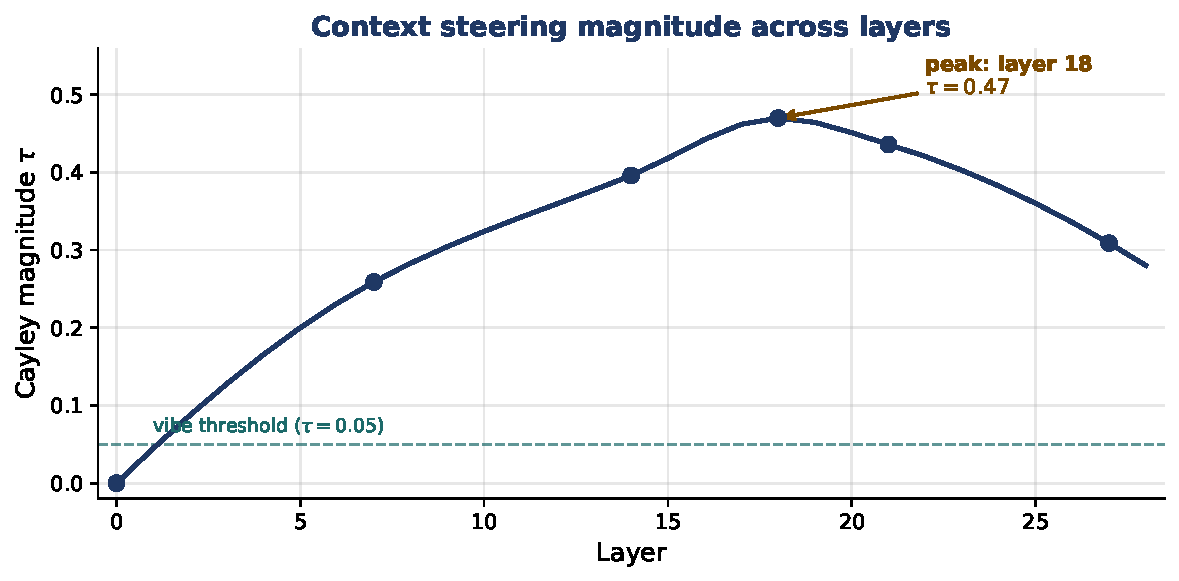
\includegraphics[width=0.8\linewidth]{figures_ga_learning/ch13_cayley_tau.pdf}
\captionof{figure}{Steering magnitude $\tau$ across layers.  The context
shifts the representation most strongly at layer~18 ($\tau = 0.47$),
well above the vibe threshold $\tau = 0.05$.  Layer~0 shows $\tau = 0$
because both prompts share the same initial embedding.}
\end{center}

\textbf{Interpretation.}
All $\tau$ values are far above the vibe threshold of $0.05$, confirming
the model \emph{is} using context.  The steering magnitude peaks at
layer~18 ($\theta = 36.5^\circ$) --- the model's representation shifts
most strongly in the middle-to-late layers.  The Cayley bivector at the
peak layer decomposes into a dominant principal plane with angle $0.33$
rad, identifying the specific 2D subspace where context rotates the
representation.

\begin{finding}
\textbf{Curvature plane shift is a stronger indicator than magnitude
change} (observed in this example).  Scalar curvature magnitude may
change by only 10--20\%, but the \emph{direction} of curvature can
shift substantially, indicating
qualitatively different computation.  This is information that scalar
summaries cannot provide --- only the bivector direction reveals it.
\end{finding}

% ────────────────────────────────────────────────────────────────────
\section{Application 2: Hallucination signatures}
\label{sec:hallucination}
% ────────────────────────────────────────────────────────────────────

\subsection{Two failure modes}

Chain-of-thought prompting can fail in two geometrically distinct ways:

\begin{enumerate}[nosep]
\item \textbf{Aleatoric confusion}: The model generates multiple
  reasoning paths that reach contradictory conclusions.  This is
  visible as high variability in the bivector directions between
  sampled chains.
\item \textbf{Systematic hallucination (mode collapse)}: All paths
  converge to the same incorrect conclusion with high confidence.
  Entropy-based methods see low dispersion and miss this failure.
  GA catches it through the \emph{plane structure} of the computation.
\end{enumerate}

\subsection{The bivector coherence diagnostic}

Given $K$ reasoning chains with embeddings $v_1, \ldots, v_K$ (unit
vectors), the \textbf{bivector coherence} is the RMS magnitude of
all pairwise bivectors:
\[
  \mathcal{C} = \sqrt{\frac{1}{\binom{K}{2}}
  \sum_{i < j} \|v_i \op v_j\|^2}
  = \sqrt{\frac{1}{\binom{K}{2}}
  \sum_{i < j} (1 - (v_i^\top v_j)^2)}
\]
Since $\|v_i \op v_j\|^2 = \sin^2\theta_{ij}$ for unit vectors,
$\mathcal{C}$ is the RMS sine of all pairwise angles:
\begin{itemize}[nosep]
\item $\mathcal{C} \approx 0$: paths are nearly collinear
  (consistent paraphrases).
\item $\mathcal{C} \approx 1$: paths span a large angular volume
  (genuine conflict).
\end{itemize}

\begin{gabox}
\textbf{Why bivectors, not cosine similarity?}  Cosine similarity
$v_i^\top v_j$ measures alignment; $\|v_i \op v_j\|$ measures the
\emph{plane spanned} by the two paths.  When all pairs span
\emph{similar} planes, the model is confused in a structured way
(same error mode).  When they span \emph{different} planes, the model
is diffusely uncertain.  The plane direction, accessible only through
the bivector, distinguishes these two cases.
\end{gabox}

\subsection{Hallucination signatures in the GA profile}

We hypothesise that hallucinations are associated with ``busy but
useless'' layers: high geometric activity (curvature, rotation) but low
dependency.  If this hypothesis holds, GA provides plane-level
diagnostics that scalar summaries cannot:

\begin{itemize}[nosep]
\item \textbf{Consistent curvature plane}: the model may be
  ``confidently wrong'' --- performing systematic but misdirected
  computation.  The holonomy bivector at high-activity layers would
  point in a consistent direction across tokens.
\item \textbf{Random curvature planes}: the model may be ``lost'' ---
  curvature directions vary across tokens without coherent structure.
  The holonomy bivectors would have low pairwise similarity.
\end{itemize}

The following experiment tests this hypothesis on a single model
and pair of prompts.  Broader validation across models, prompt types,
and evaluation benchmarks is needed to establish these as reliable
diagnostics.

\subsection{Experiment: factual vs.\ confabulation prompt}

We compare the full GA profile for two prompts on Qwen2.5-7B:
\begin{itemize}[nosep]
\item \textbf{Factual}: ``The Eiffel Tower is a wrought iron lattice
  tower in Paris France''
\item \textbf{Confabulation}: ``The underwater city of Atlantis was
  discovered in 2019 near the coast of''
\end{itemize}

\begin{center}
\renewcommand{\arraystretch}{1.3}\small
\begin{tabular}{@{}l r r@{}}
\toprule
\textbf{Metric} & \textbf{Factual} & \textbf{Confabulation} \\
\midrule
Mean rotation angle & 6.78 & 7.50 \\
Max rotation angle & 8.85 & 9.96 \\
$D_{\text{total}}$ & 3.13 & 0.75 \\
$H(D)$ (entropy) & 2.04 & 2.36 \\
$C_{\text{acc}}$ & 7587 & 8826 \\
Concentration & 0.221 & 0.216 \\
\bottomrule
\end{tabular}
\end{center}

\begin{center}
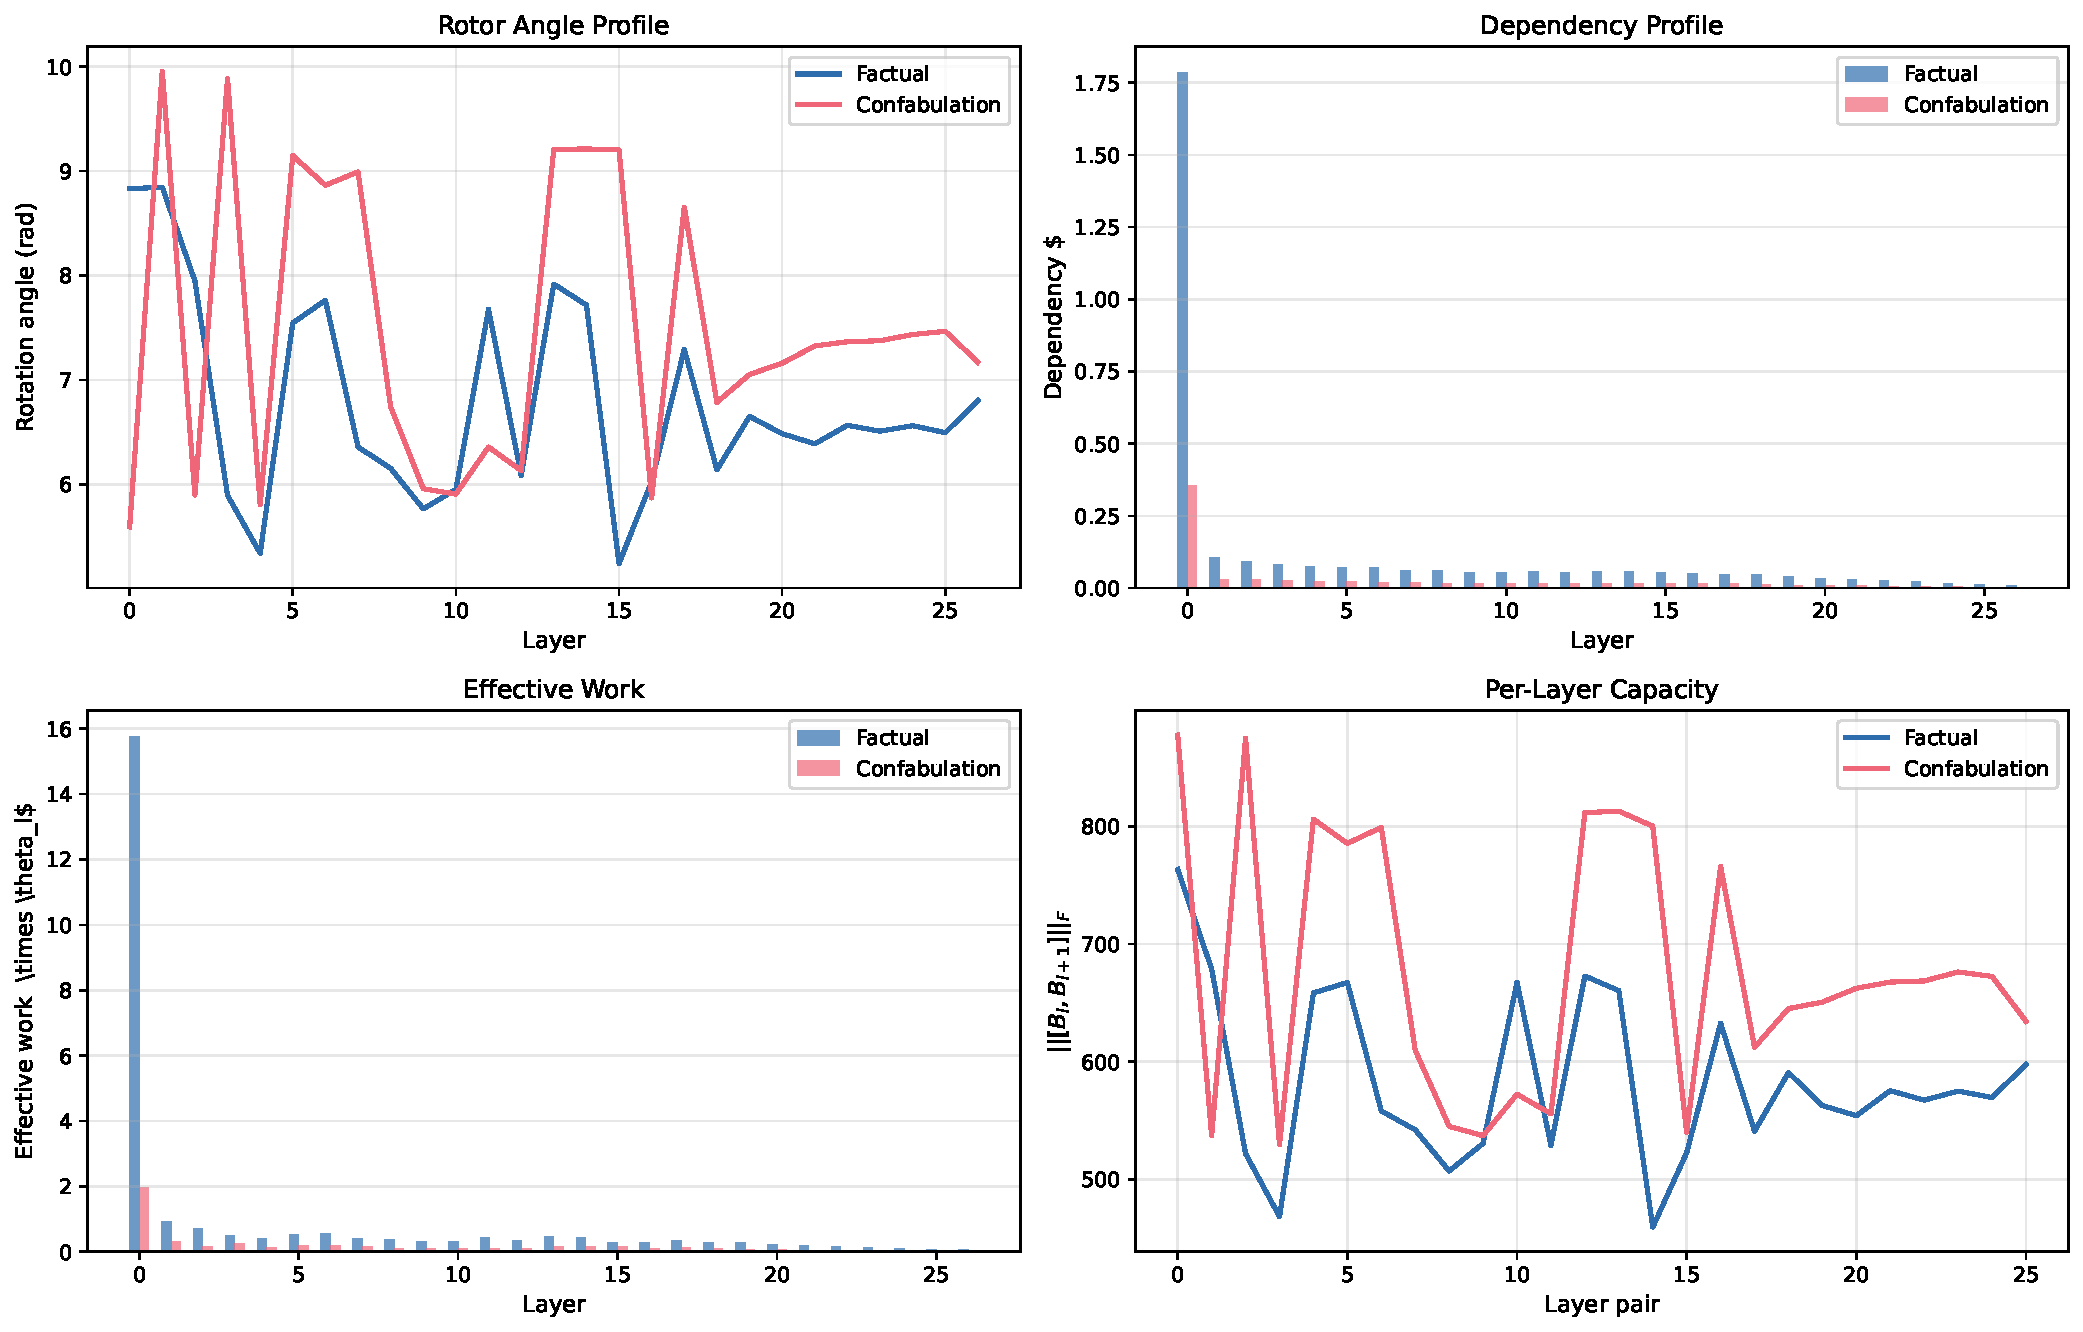
\includegraphics[width=0.95\linewidth]{figures_ga_learning/ch13_hallucination.pdf}
\captionof{figure}{Geometric profile comparison: factual (blue) vs.\
confabulation (red).  Top-left: the confabulation prompt produces
\emph{larger} rotation angles.  Top-right: but \emph{much smaller}
dependency --- the model does not rely on these rotations.  Bottom-left:
effective work is concentrated in layer~0 for the factual prompt.
Bottom-right: capacity is higher for confabulation.}
\end{center}

\textbf{Interpretation.}
The confabulation prompt has \textbf{higher geometric activity}
(mean rotation $7.50$ vs $6.78$, capacity $8826$ vs $7587$) but
\textbf{4$\times$ lower dependency} ($D_{\text{total}} = 0.75$ vs
$3.13$).  This is the ``busy but useless'' signature: the model's
internal rotations are large and complex, but the output barely
depends on them.  The model is churning through representations
without arriving at a grounded answer.

The factual prompt concentrates effective work in the earliest layers
--- the model quickly builds a confident representation.  The
confabulation prompt spreads computation more evenly (higher entropy
$2.36$ vs $2.04$), indicating the model never settles on a coherent
geometric path.

\begin{finding}
\textbf{Metric anisotropy complements rotational diagnostics}
(observed in this example).
The condition number $\kappa_G$ of the Gram matrix
$G_{ij} = v_i^\top v_j$ measures spectral concentration.  In
Qwen2.5-7B, factual prompts produce more spectrally concentrated
paths (low effective rank) than confabulations.  High $\kappa_G$ with
low $\mathcal{C}$ would be a \emph{warning sign}: apparent consistency
that may be a metric artefact rather than genuine agreement.  Whether
these patterns generalise requires further investigation.
\end{finding}

\subsection{The Binet--Cauchy cosine: detecting causal inversions}

Bivector coherence tells you whether reasoning \emph{paths} agree with
each other.  But a model can also fail in a subtler way: the logical
\emph{direction} of reasoning can be reversed --- a conclusion appears
before its premise, or a cause follows its effect.  This is a
\textbf{causal inversion}, and detecting it requires an oriented
measure.

The \textbf{Binet--Cauchy cosine} (BCcos) provides exactly this.
Consider two pairs of unit vectors:
\begin{itemize}[nosep]
\item $(u_i, u_{i+1})$: consecutive reasoning-step embeddings
  (the model's trajectory).
\item $(c_q, c_{\text{ctx}})$: query and context direction
  (the expected flow of information).
\end{itemize}

Form the $2 \times 2$ matrix of their inner products:
\[
  S = \begin{pmatrix}
    u_i^\top c_q & u_i^\top c_{\text{ctx}} \\
    u_{i+1}^\top c_q & u_{i+1}^\top c_{\text{ctx}}
  \end{pmatrix}
\]

\begin{gabox}
\textbf{Binet--Cauchy cosine.}
\[
  \text{BCcos}(u_i, u_{i+1}; c_q, c_{\text{ctx}})
  = \frac{\det S}{\|u_i \op u_{i+1}\| \; \|c_q \op c_{\text{ctx}}\|
    + \epsilon}
\]
The numerator $\det S$ is a \textbf{signed oriented area}: it equals
the inner product between the bivectors $u_i \op u_{i+1}$ and
$c_q \op c_{\text{ctx}}$.  The denominator normalises by the product
of their areas.
\end{gabox}

\paragraph{Why this is a GA concept.}
The determinant $\det S = (u_i^\top c_q)(u_{i+1}^\top c_{\text{ctx}})
- (u_i^\top c_{\text{ctx}})(u_{i+1}^\top c_q)$ is precisely the
contraction of two bivectors:
$\langle u_i \op u_{i+1}, \, c_q \op c_{\text{ctx}} \rangle$.  In
GA language, BCcos measures whether the \emph{plane of the model's
reasoning trajectory} is aligned with the \emph{plane of the expected
information flow}.

\paragraph{Three regimes of BCcos.}
\begin{itemize}[nosep]
\item \textbf{BCcos $\approx +1$}: the reasoning trajectory is aligned
  with the expected information flow (correct causal direction).
\item \textbf{BCcos $\approx 0$}: the trajectory is orthogonal to
  the expected flow (irrelevant computation).
\item \textbf{BCcos $\ll 0$ (strongly negative)}: the trajectory is
  \emph{reversed} --- a causal inversion.  The model's reasoning
  flows opposite to the expected direction.
\end{itemize}

\begin{keyidea}
Cosine similarity can tell you whether two vectors are aligned, but it
cannot detect \emph{causal inversions} --- for that, you need an
\textbf{oriented} measure that is sensitive to the \emph{order} of the
vectors.  The determinant of $S$ provides this orientation through the
wedge product.  This is information that no scalar similarity measure
can capture.
\end{keyidea}

% ────────────────────────────────────────────────────────────────────
\section{Application 3: Plane-specific steering}
\label{sec:steering}
% ────────────────────────────────────────────────────────────────────

\subsection{The directional--radial decomposition}

Every whitened hidden state admits a polar factorisation:
\[
  \widetilde{H}^{(l,t)} = r^{(l,t)} \, \hat{H}^{(l,t)},
  \qquad \|\hat{H}^{(l,t)}\| = 1
\]
A steering perturbation $\delta$ decomposes into two orthogonal
components:
\begin{align*}
  \delta_{\text{angular}} &= \delta - (\delta^\top \hat{H})\,\hat{H}
  &&\text{(tangent to the sphere: changes direction)} \\
  \delta_{\text{radial}} &= (\delta^\top \hat{H})\,\hat{H}
  &&\text{(normal to the sphere: changes energy)}
\end{align*}
By Pythagoras:
$\|\delta\|^2 = \|\delta_{\text{angular}}\|^2 +
\|\delta_{\text{radial}}\|^2$.

\begin{transformer}
The angular component corresponds to \textbf{grade-2} (rotation)
and the radial component to \textbf{grade-0} (scaling).  This
decomposition is the single-vector analogue of the versor decomposition
$T^{(l)} = \rotor{l}\metric{l}$ from Chapter~\ref{chap:versor}.
\end{transformer}

\subsection{Why the rotation plane matters}

The versor decomposition tells us that inter-layer dynamics are
\textbf{metric-dominated}: the symmetric factor $\metric{l}$
contributes $\sim$94--97\% of the transition operator's Frobenius norm,
while the rotation factor $\rotor{l}$ contributes only $\sim$3--6\%.

This has a profound consequence for intervention design.  A steering
perturbation $\delta^{(l)}$ applied at layer $l$ propagates to layer
$l+1$ approximately as:
\[
  \delta_{\text{propagated}}^{(l+1)} \approx
  T^{(l)} \, \delta^{(l)} = \rotor{l} \metric{l} \, \delta^{(l)}
\]
Because $\metric{l}$ dominates, the propagated perturbation is shaped
primarily by the \emph{stretching directions} of $\metric{l}$, not
by the rotation $\rotor{l}$.  A purely angular intervention at one
layer acquires a radial component at the next:
\[
  \metric{l}\,\delta_{\text{angular}}^{(l)} =
  \underbrace{(\metric{l}\delta_{\text{angular}})_{\text{angular}}}_{\text{survives}}
  + \underbrace{(\metric{l}\delta_{\text{angular}})_{\text{radial}}}_{\text{generated by stretching}}
\]

\begin{pitfall}
\textbf{Per-layer isometry does not guarantee end-to-end isometry.}
A purely rotational intervention (e.g., Cayley steering) is exactly
isometric at each layer.  But the model's metric-dominated dynamics
convert angular perturbations into radial ones.  Over 28 layers,
purely angular purity degrades substantially.  Dense addition, which
appears geometrically crude, can achieve higher end-to-end angular
purity because $|v^\top \hat{H}| \sim \mathcal{O}(1/\sqrt{k})$ in
high dimensions, making the perturbation naturally tangential.
\end{pitfall}

\subsection{The steering recipe}

\begin{keyidea}
\textbf{Plane-specific steering.}
Instead of modifying all directions at a target layer, intervene only
in the \textbf{principal rotation plane}:
\begin{enumerate}[nosep]
\item Identify target layers by effective work $D_l \cdot \theta^{(l)}$
  (Chapter~\ref{chap:dependency}).
\item Extract the dominant bivector plane $\hat{B}^{(l)}$ at each
  target layer.  Let $(u_1, u_2)$ be its spanning eigenvectors.
\item Project $\metric{l}$ into the 2D subspace:
  $\metric{l}_{\text{plane}} = U_2^\top \metric{l} U_2$ where
  $U_2 = [u_1, u_2]$.
\item Modify only the eigenvalues of $\metric{l}_{\text{plane}}$
  (amplify or suppress), leaving all other directions unchanged.
\end{enumerate}
This is a rank-2 intervention in a $k$-dimensional space --- maximally
targeted.  The intervention respects the model's own geometry: it acts
in the plane where the model already performs its rotation.
\end{keyidea}

\begin{lstlisting}[caption={Identifying steering targets}]
# Effective work per layer
eff_work = result.dependency_profile * result.angles[:n]

# Top-2 steering targets
top_layers = np.argsort(eff_work)[-2:][::-1]

for l in top_layers:
    vd = rf.decompositions[l]
    plane = vd.bivector.principal_planes(n_planes=1)[0]
    print(f"Layer {l}: D={result.dependency_profile[l]:.4f}, "
          f"theta={result.angles[l]:.4f}, "
          f"plane_angle={plane['angle']:.4f}")
    # plane['eigvecs'] gives the 2D subspace for intervention
\end{lstlisting}

\subsection{Experiment: identifying steering targets}

Running the steering recipe on Qwen2.5-7B with the factual prompt:

\begin{center}
\renewcommand{\arraystretch}{1.3}\small
\begin{tabular}{@{}r r r r r@{}}
\toprule
\textbf{Layer} & $D_l$ & $\theta^{(l)}$ &
  $D_l \times \theta^{(l)}$ & \textbf{Top plane angle} \\
\midrule
0 & 1.786 & 8.831 & 15.769 & 3.131 \\
1 & 0.106 & 8.845 & 0.935 & 3.135 \\
2 & 0.090 & 7.948 & 0.717 & 3.131 \\
\bottomrule
\end{tabular}
\end{center}

Layer~0 dominates overwhelmingly: its effective work ($15.8$) is
$17\times$ larger than layer~1's ($0.94$).  This layer is the primary
steering target.

\paragraph{Plane independence.}
The bivector similarity between the top-3 layers is near zero:
\begin{center}
\renewcommand{\arraystretch}{1.3}\small
\begin{tabular}{@{}l r@{}}
\toprule
\textbf{Layer pair} & \textbf{Bivector similarity} \\
\midrule
Layers 0 vs 1 & $+0.005$ \\
Layers 0 vs 2 & $+0.027$ \\
Layers 1 vs 2 & $-0.026$ \\
\bottomrule
\end{tabular}
\end{center}

\textbf{Interpretation.}
The near-zero similarities confirm that each layer rotates in an
essentially \emph{independent} plane.  Steering at layer~0 will not
interfere with the rotation at layers 1 or 2.  At each target layer,
the top-3 principal planes each carry $\sim$25\% of the rotation
weight, indicating compound (multi-plane) rotations.  A plane-specific
intervention at layer~0 would target the dominant 2D subspace,
modifying only 2 of $k$ dimensions --- a maximally surgical intervention.

\subsection{Comparison of steering methods}

The following table summarises the geometric character of common
steering approaches:

\begin{center}
\renewcommand{\arraystretch}{1.4}\small
\begin{tabular}{@{}L{3cm} L{3.5cm} L{4cm}@{}}
\toprule
\textbf{Method} & \textbf{Steering type} & \textbf{GA interpretation} \\
\midrule
Dense addition & $\delta = \alpha\,v$ (constant) &
  Naturally angular in high-$k$ \\
Cayley/Rodrigues & $\delta = A\hat{H}$ (rotation) &
  Exactly grade-2 per layer \\
Sparse activation & $\delta = \lambda\,\Delta z$ &
  Acts on monosemantic features \\
Plane-specific & Modify $\metric{l}$ in 2D &
  Targeted grade-0 in one plane \\
\bottomrule
\end{tabular}
\end{center}

\begin{finding}
\textbf{Rotation as a mechanism of semantic steering} (interpretive
hypothesis, supported by initial experiments).
The examples in this chapter suggest that context influence in language
models is a rotational phenomenon.  The Cayley bivector provides a
unified representation: its magnitude detects vibing, its direction
diagnoses the semantic category of context influence, and its
associated rotation enables active intervention.  In prior ablation
studies on Qwen2.5-7B, random rotations catastrophically fail (0\%
context-following), while learned rotations succeed (83\%), and
scaling alone has no effect --- consistent with the antisymmetric
(bivector) component carrying the semantically meaningful signal.
Establishing the generality of this finding across models and domains
remains important future work.
\end{finding}

\begin{tryit}
\textbf{Notebook: Chapter 13.}
\begin{enumerate}[nosep]
\item Run the context-ignoring detection on a factual question with and
  without a relevant paragraph.  Does the curvature plane shift?
\item Generate the GA summary plot for a prompt you suspect will produce
  a hallucination.  Look for the ``busy but useless'' layers.
\item Identify the top-2 steering targets (layer + plane) for a given
  prompt.
\end{enumerate}

\medskip
\textbf{Sample output} --- the GA summary plot brings together all four
diagnostic dimensions in a single view:

\begin{center}
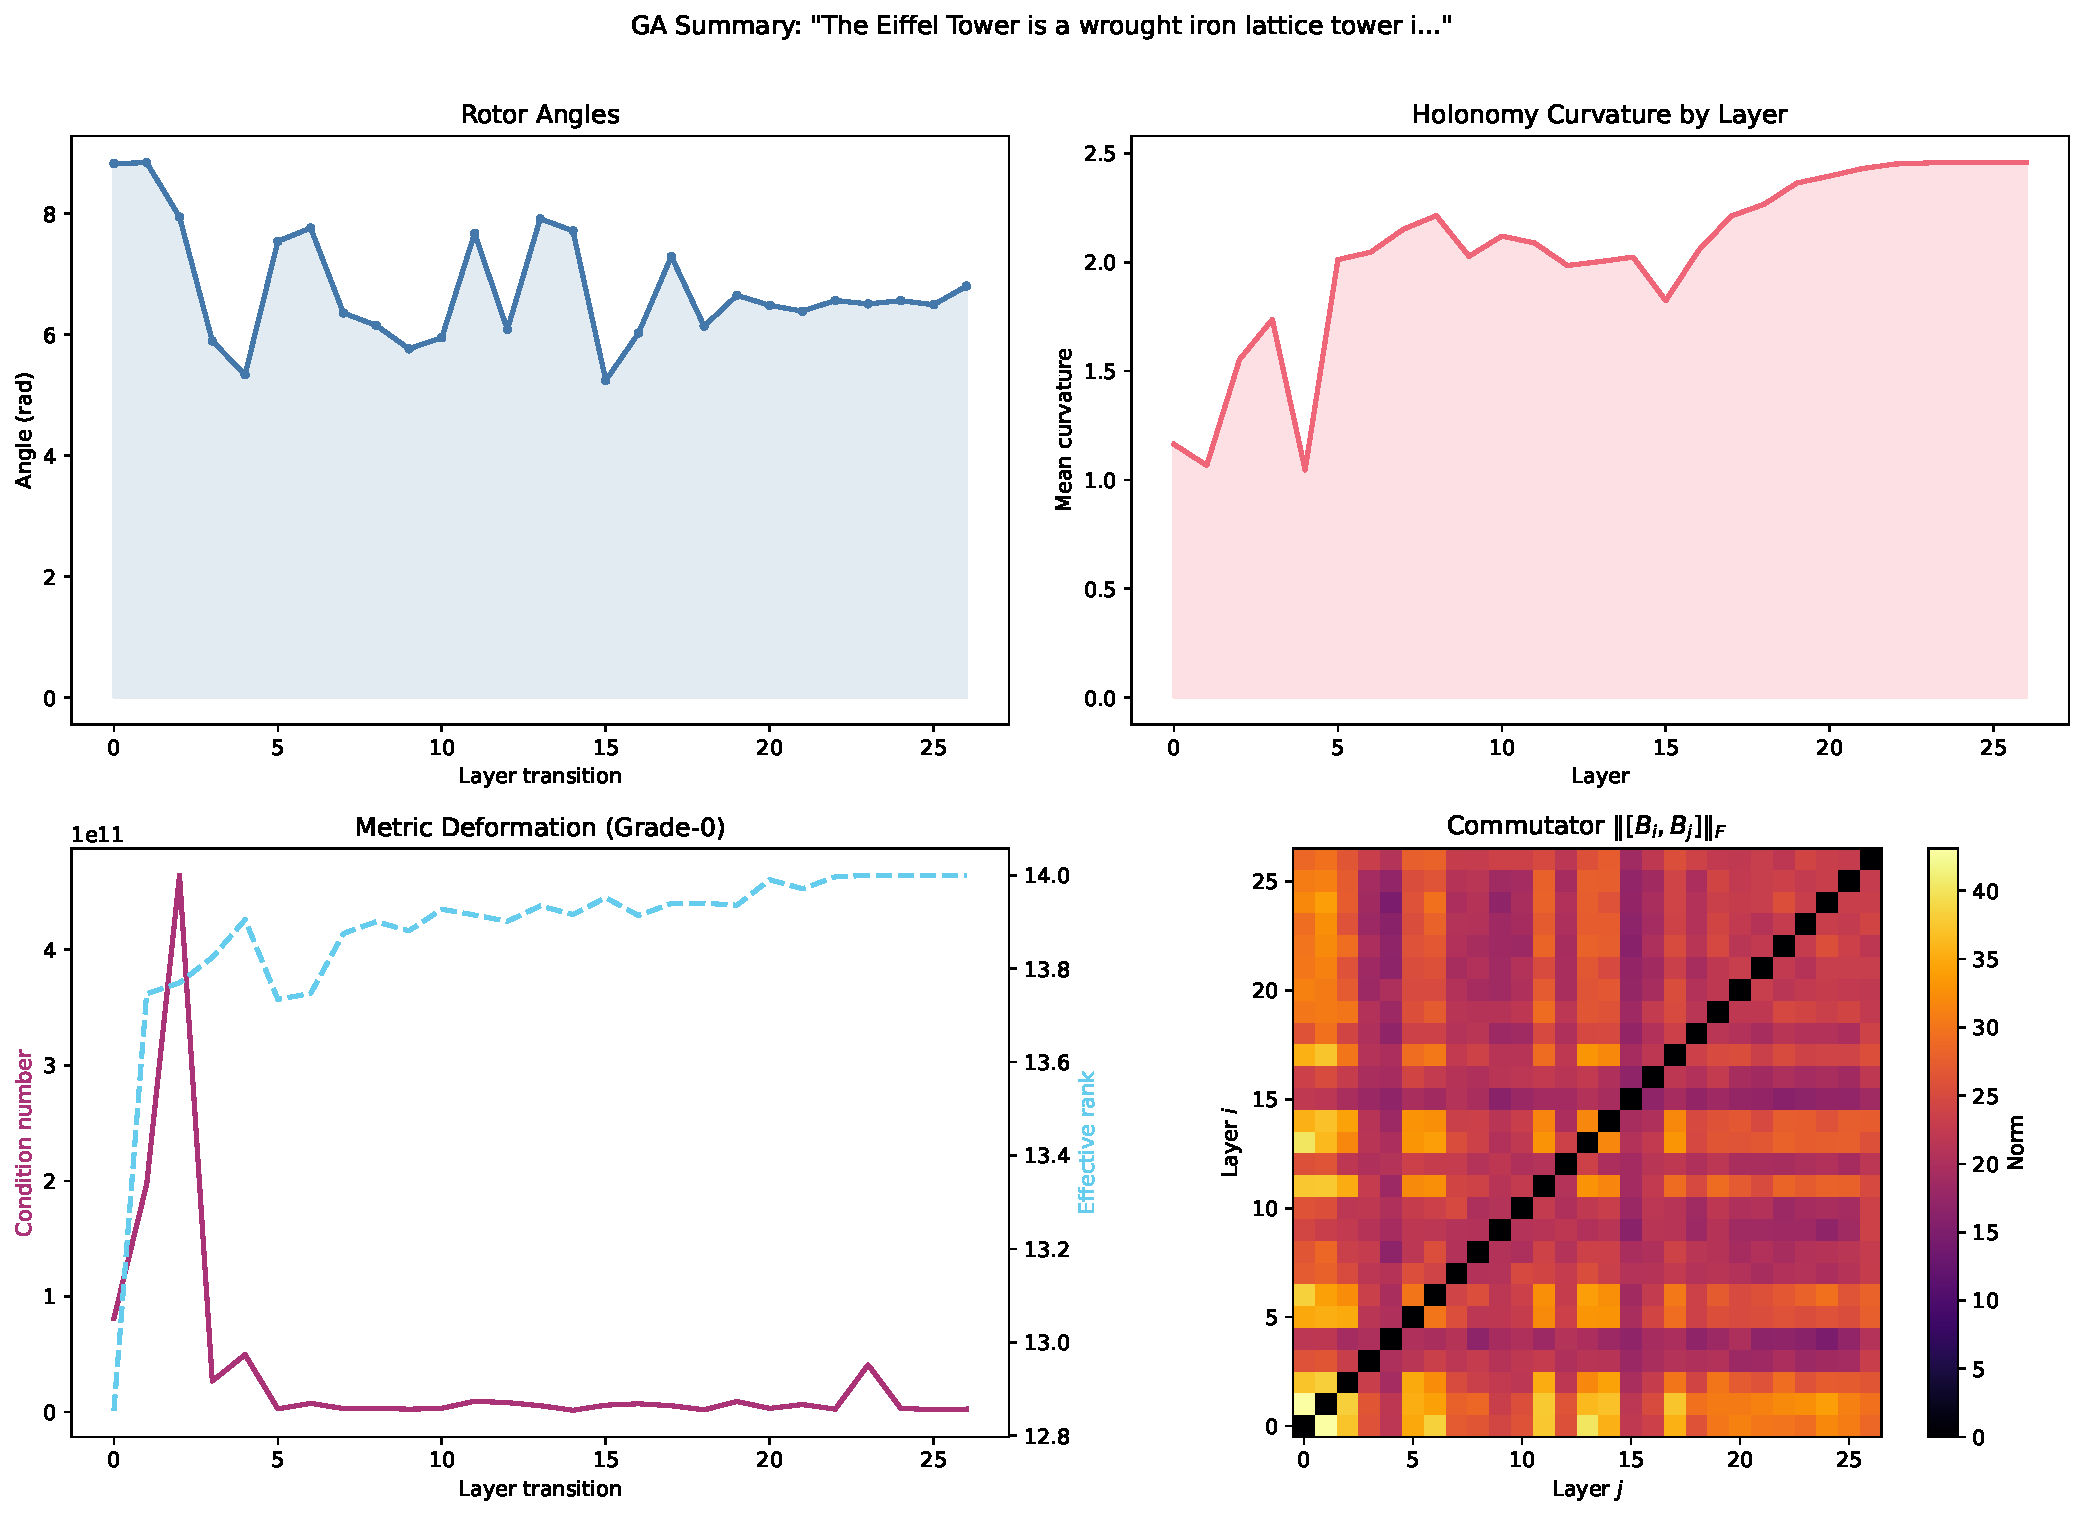
\includegraphics[width=0.95\linewidth]{figures_ga_learning/ch13_ga_summary.pdf}
\captionof{figure}{4-panel GA summary for Qwen2.5-7B on a 14-token prompt.
Top-left: rotor angles.  Top-right: plane similarity.
Bottom-left: curvature map.  Bottom-right: capacity contributions.}
\end{center}
\end{tryit}


% ══════════════════════════════════════════════════════════════════════════════
\chapter{What Geometric Algebra Gave Us}
\label{chap:conclusion}
% ══════════════════════════════════════════════════════════════════════════════

\section{The journey}

You started with vectors and the dot product.  You now have:

\begin{center}
\renewcommand{\arraystretch}{1.5}\small
\begin{tabular}{@{}L{3cm} L{4cm} L{4cm}@{}}
\toprule
\textbf{Chapter} & \textbf{GA concept} & \textbf{Transformer insight} \\
\midrule
1--2 & Vectors, geometric product & Hidden states encode both alignment
  and plane information \\
3 & Bivectors & Layer rotations have principal planes, not just
  magnitudes \\
4 & Orthonormal frames & Whitening establishes the metric for valid GA \\
5 & Rotors & Layer transitions are rotations with explicit planes \\
6 & Versor decomposition & Grade-0 (stretch) vs.\ grade-2 (rotation) \\
7 & Principal planes & Rotation plane evolution across the network \\
8 & Eigenvalues & Grade-0 dominates control; late layers are highly
  selective \\
9 & Commutators & Non-commutativity lives in specific planes \\
10 & Holonomy & Curvature has a direction, not just a magnitude \\
11 & Capacity & Decompose computational complexity by plane \\
12 & Dependency + bivectors & Identify the planes that matter \\
13 & Applications & Diagnose and steer via plane-specific interventions \\
\bottomrule
\end{tabular}
\end{center}

\section{What was invisible before}

Scalar summaries ($\|U - I\|_F$, $\|[A_i, A_j]\|_F$, $\|\Omega - I\|_F$)
tell you \emph{how much}.  GA tells you \emph{how much} and
\emph{in which direction}.  Specifically:

\begin{enumerate}[nosep]
\item Which planes each layer rotates in.
\item Which planes the curvature acts in.
\item Which planes different layers fail to commute in.
\item Which planes the model's output depends on.
\end{enumerate}

None of this information is accessible from norms alone.  It requires
the full bivector.

\section{Where to go next}

\begin{enumerate}
\item \textbf{Higher grades.}  We used only grades 0 and 2.  Do
  trivectors (grade 3) carry meaningful information about three-layer
  interactions?

\item \textbf{Conformal GA.}  The conformal model $\mathrm{Cl}(k+1,1)$
  adds translations to the algebra.  Could this unify residual
  connections (translations) with rotations (rotors)?

\item \textbf{GA in training dynamics.}  How does the bivector field
  evolve during pre-training?  Do specific planes emerge at specific
  training stages?

\item \textbf{Multimodal models.}  When vision and language tokens
  interact, do they occupy different rotation planes?

\item \textbf{Projective GA.}  $\mathrm{Cl}(k,0,1)$ naturally handles
  the affine structure of residual connections.
\end{enumerate}

\section{Further reading}

\begin{itemize}[nosep]
\item Doran and Lasenby, \emph{Geometric Algebra for Physicists}
  (Cambridge, 2003).  The most accessible GA introduction.
\item Dorst, Fontijne, and Mann, \emph{Geometric Algebra for Computer
  Science} (Morgan Kaufmann, 2007).  Practical and code-oriented.
\item Lounesto, \emph{Clifford Algebras and Spinors} (Cambridge, 2001).
  The mathematical reference.
\item Sudjianto and Zhang, \emph{Layer--Time Geometry: How Language
  Models Process Information} (2026).  The first-edition linear algebra
  treatment.
\item Fang, Li, and Sudjianto, \emph{Design and Modeling for Computer
  Experiments} (Chapman \& Hall/CRC, 2006).  Background on DOE
  methodology.
\end{itemize}


% ══════════════════════════════════════════════════════════════════════════════
% APPENDICES
% ══════════════════════════════════════════════════════════════════════════════
\appendix


% ══════════════════════════════════════════════════════════════════════════════
\chapter{Transformers: A Primer}
\label{app:transformers}
% ══════════════════════════════════════════════════════════════════════════════

This appendix provides the transformer background needed for the book.
No prior ML knowledge is assumed; we build from first principles.

\section{What is a language model?}

A language model is a function that, given a sequence of words (tokens),
predicts the next word.  ``The capital of France is'' $\to$ ``Paris.''
Internally, the model converts each token into a vector, transforms
those vectors through many layers of computation, and reads out the
prediction from the final layer.  The key objects for us are the
\textbf{hidden states} --- the intermediate vectors at each layer.

\section{Tokens and embeddings}

Before processing, text is split into \textbf{tokens} (roughly
word-pieces).  Each token is assigned a vector $H^{(0,t)} \in
\mathbb{R}^p$ from a learned \textbf{embedding table}.  The integer
$t$ indexes the token position; $p$ is the \textbf{hidden dimension}
(e.g., $p = 3584$ for Qwen2.5-7B).  These initial vectors are the
starting point for all subsequent computation.

\section{The architecture}

A transformer consists of $L$ identical layers stacked sequentially.
Each layer transforms the hidden state $H^{(l,t)} \to H^{(l+1,t)}$.
Each layer has two main sub-components:

\begin{enumerate}[nosep]
\item \textbf{Self-attention}: Each token ``looks at'' all other tokens
  and computes a weighted average of their representations.  This is
  the mechanism by which tokens communicate --- information from one
  position can influence another.  Attention enables context-dependent
  processing: the same word is represented differently depending on
  its neighbours.

\item \textbf{Feed-forward network (MLP)}: A two-layer neural network
  applied to each token independently.  This is the model's
  ``thinking'' step for each token, combining and transforming
  features without inter-token communication.
\end{enumerate}

Both sub-components use \textbf{residual connections}: the output is
added to the input, $H^{(l+1)} = H^{(l)} + \Delta H^{(l)}$.  This
means the hidden state accumulates changes layer by layer rather than
being overwritten.  \textbf{Layer normalization} stabilizes the scale
of representations.

The hidden state $H^{(l, t)} \in \mathbb{R}^p$ at layer $l$ and token
position $t$ is the model's internal representation --- the central
object of this book.

\section{The hidden-state grid}

The full set of hidden states forms a two-dimensional grid:
\begin{itemize}[nosep]
\item \textbf{Layer axis}: $l = 0, 1, \ldots, L-1$, from input
  embedding to final representation.
\item \textbf{Token axis}: $t = 0, 1, \ldots, T-1$, from the first
  token to the last.
\end{itemize}
Each grid point holds a $p$-dimensional vector.  This $(L \times T)$
grid is the ``laboratory'' we study with GA.  Moving along the layer
axis corresponds to the model's processing depth; moving along the
token axis corresponds to the model's processing breadth.

\section{Autoregressive prediction}

GPT-style models predict the next token given all preceding tokens:
$P(x_t \mid x_{<t})$.  The final hidden state $H^{(L-1, t)}$ is
projected to vocabulary logits via a learned linear map, and the
highest-probability token is selected.  The \textbf{score}
$s(x, u)$ of a token $u$ at the end of text $x$ is the logit
assigned to $u$ --- this is what the dependency gradient
(Chapter~\ref{chap:dependency}) differentiates through.

\section{What gradients measure}

A \textbf{gradient} is the derivative of a scalar output with respect
to an input.  If the model's score for token ``Paris'' is
$s$, then $\partial s / \partial H^{(l,t)}$ is a vector pointing in
the direction of hidden-state change that most increases the score for
``Paris'' at layer~$l$, token~$t$.  Its magnitude tells you how
\emph{sensitive} the output is to changes at that point.

In this book, we use gradients to compute \textbf{dependency density}
(Chapter~\ref{chap:dependency}): $D_{l,t} = \|\partial s / \partial
H^{(l,t)}\|$.  This tells us which layers and tokens matter most for
the model's prediction --- without altering the model or its output.

\section{The models we study}

\begin{itemize}[nosep]
\item \textbf{Qwen2.5-7B}: 28 layers, hidden dimension 3584, 7 billion
  parameters.  Our primary laboratory throughout the book.
\item \textbf{Qwen2.5-32B}: 64 layers, hidden dimension 5120, 32
  billion parameters.  Used for scaling comparisons.
\item \textbf{DeepSeek-R1-Distill-Qwen-7B}: same architecture as
  Qwen-7B, distilled from a larger reasoning model.  Used to study
  how training objective affects geometric structure.
\end{itemize}

All models are freely available on Hugging Face and can be loaded with
a single line of code (see the Preface).  A GPU with 16\,GB of memory
is sufficient for the 7B models.


% ══════════════════════════════════════════════════════════════════════════════
\chapter{GA from Scratch}
\label{app:ga-formal}
% ══════════════════════════════════════════════════════════════════════════════

This appendix builds up Geometric Algebra from first principles.
If you have taken a linear algebra course and are comfortable with
vectors, dot products, and matrices, you have everything you need.
We introduce one idea at a time, with small examples you can verify
by hand.

\section{The problem GA solves}

Linear algebra gives you two operations on vectors: the \textbf{dot
product} $a \ip b$ (a scalar) and the \textbf{cross product}
$a \times b$ (a vector, but only in 3D).  The dot product tells you
about alignment; the cross product tells you about the plane the two
vectors span.

But the cross product is a 3D accident.  In $\mathbb{R}^{256}$ (the
kind of space we encounter inside transformers), there is no cross
product.  Yet we still want to talk about the plane that two vectors
define, the rotation that maps one vector to another, and how
rotations compose.

Geometric Algebra solves this by introducing a single product --- the
\textbf{geometric product} --- that captures both alignment and plane
information in any dimension.  Everything else follows.

\section{The geometric product: one rule}

Start with a vector space $V = \mathbb{R}^k$ equipped with the
standard inner product.  The \textbf{geometric product} is an
associative product on vectors defined by one rule:

\begin{gabox}
\textbf{The fundamental identity.}  For any vector $v$:
\[
  v \, v = v \ip v = \|v\|^2
\]
The geometric product of a vector with itself is its squared length.
\end{gabox}

That's it.  This single rule, combined with associativity and
distributivity, generates the entire algebra.

Let's see what this implies.  Pick an orthonormal basis
$e_1, e_2, \ldots, e_k$ (so $e_i \ip e_j = \delta_{ij}$).
From the fundamental identity:
\[
  e_i \, e_i = e_i \ip e_i = 1
\]

Now consider the product $e_1 \, e_2$.  We can derive its properties.
Compute $(e_1 + e_2)^2$ in two ways:

\textbf{By the fundamental identity:}
$(e_1 + e_2)^2 = \|e_1 + e_2\|^2 = 2$

\textbf{By expanding:}
$(e_1 + e_2)^2 = e_1 e_1 + e_1 e_2 + e_2 e_1 + e_2 e_2
= 1 + e_1 e_2 + e_2 e_1 + 1 = 2 + e_1 e_2 + e_2 e_1$

Comparing: $e_1 e_2 + e_2 e_1 = 0$, so

\begin{gabox}
\textbf{Anti-commutativity of orthogonal vectors.}
\[
  e_i \, e_j = -e_j \, e_i \qquad (i \neq j)
\]
Orthogonal vectors anti-commute under the geometric product.
\end{gabox}

For general vectors $a$ and $b$, the geometric product decomposes as:
\[
  a \, b = \underbrace{a \ip b}_{\text{scalar (grade-0)}}
         + \underbrace{a \op b}_{\text{bivector (grade-2)}}
\]
The \textbf{inner product} $a \ip b$ is the familiar dot product.
The \textbf{outer product} $a \op b$ is something new: a
\emph{bivector}, which represents the oriented plane spanned by $a$
and $b$.

\paragraph{A small example.}
In $\mathbb{R}^3$, let $a = 3e_1 + e_2$ and $b = e_1 + 2e_2$.  Then:
\begin{align*}
  a \ip b &= 3 \cdot 1 + 1 \cdot 2 = 5 \\
  a \op b &= (3 \cdot 2 - 1 \cdot 1)\, e_1 \op e_2
           = 5 \, e_1 \op e_2
\end{align*}
So $a\,b = 5 + 5\,e_1 \op e_2$.
The scalar part says the vectors are partially aligned.  The bivector
part says they span an area of 5 in the $e_1 e_2$ plane.

\section{The Clifford algebra $\mathrm{Cl}(k, 0)$}

The algebra generated by all products of basis vectors $e_1, \ldots, e_k$
under the geometric product is the \textbf{Clifford algebra}
$\mathrm{Cl}(k, 0)$.  The ``$(k, 0)$'' means $k$~dimensions with a
positive-definite metric (all basis vectors square to $+1$).

The distinct basis elements are:
\begin{center}
\renewcommand{\arraystretch}{1.3}\small
\begin{tabular}{@{}l l l l@{}}
\toprule
\textbf{Grade} & \textbf{Basis elements} & \textbf{Count} & \textbf{Name} \\
\midrule
0 & $1$ & $\binom{k}{0} = 1$ & Scalars \\
1 & $e_1, e_2, \ldots, e_k$ & $\binom{k}{1} = k$ & Vectors \\
2 & $e_1 e_2, \; e_1 e_3, \; \ldots$ & $\binom{k}{2} = \frac{k(k-1)}{2}$ & Bivectors \\
3 & $e_1 e_2 e_3, \; \ldots$ & $\binom{k}{3}$ & Trivectors \\
$\vdots$ & $\vdots$ & $\vdots$ & $\vdots$ \\
$k$ & $e_1 e_2 \cdots e_k$ & $1$ & Pseudoscalar \\
\bottomrule
\end{tabular}
\end{center}

The total dimension is $\sum_{r=0}^k \binom{k}{r} = 2^k$.  A general
element of $\mathrm{Cl}(k, 0)$ is a \textbf{multivector}: a sum of
components across different grades.

For $k = 3$: $\mathrm{Cl}(3,0)$ has dimension $2^3 = 8$, with
1~scalar, 3~vectors, 3~bivectors, and 1~pseudoscalar.

For $k = 256$ (the whitened dimension used in this book): $\mathrm{Cl}(256, 0)$
has dimension $2^{256}$, an astronomically large space.  But we only
ever use grades 0, 1, and 2 --- scalars, vectors, and bivectors --- which
is a subspace of dimension $1 + 256 + 32{,}640 = 32{,}897$.

\section{Blades and multivectors}

A \textbf{blade} is a grade-$r$ element that can be written as a single
outer product:
\[
  B_r = v_1 \op v_2 \op \cdots \op v_r
\]

A blade represents an oriented $r$-dimensional subspace.  For grade-2
(bivectors), a blade is a single oriented plane.  A general bivector
may be a sum of blades --- this happens when a rotation involves
multiple planes simultaneously.

\paragraph{Example: simple vs compound bivectors.}
\begin{itemize}[nosep]
\item $B = 3 \, e_1 \op e_2$ is a \textbf{simple} bivector (a blade):
  it represents one plane.
\item $B = 2 \, e_1 \op e_2 + 5 \, e_3 \op e_4$ is a \textbf{compound}
  bivector: it involves two independent planes.  This cannot be written
  as a single $v_1 \op v_2$.
\end{itemize}

In 3D, every bivector is simple (there is only one independent plane).
In 4D and above, compound bivectors exist and are common.  In the
256-dimensional space of transformer hidden states, layer transition
bivectors are highly compound --- they involve dozens of active planes.
This is where the ``principal plane decomposition'' from Chapter~3
becomes essential.

\section{Rotors: the GA way to rotate}

A \textbf{rotor} is an even-grade element (scalar + bivector + \ldots)
that satisfies $R\rev{R} = 1$, where $\rev{R}$ is the \textbf{reverse}
(reverse the order of all vector factors).

The simplest rotor rotates by angle $\theta$ in the plane of unit
bivector $\hat{B}$:
\[
  R = \exp\!\left(-\frac{\hat{B}\theta}{2}\right)
    = \cos\!\left(\frac{\theta}{2}\right)
    - \hat{B}\,\sin\!\left(\frac{\theta}{2}\right)
\]

Why the half angle?  Because a rotor acts on a vector $v$ via the
\textbf{sandwich product}:
\[
  v' = R \, v \, \rev{R}
\]
The two factors of $R$ each contribute $\theta/2$, giving a total
rotation of $\theta$.

\paragraph{Example in $\mathbb{R}^3$.}
To rotate $e_1$ by $90^\circ$ in the $e_1 e_2$ plane:
\begin{align*}
  R &= \cos(45^\circ) - e_1 e_2 \sin(45^\circ)
     = \frac{\sqrt{2}}{2}(1 - e_1 e_2) \\
  R \, e_1 \, \rev{R}
    &= \frac{1}{2}(1 - e_1 e_2)\, e_1 \,(1 + e_1 e_2) \\
    &= \frac{1}{2}(e_1 - e_1 e_2 e_1)(1 + e_1 e_2) \\
    &= \frac{1}{2}(e_1 + e_2)(1 + e_1 e_2) \\
    &= e_2 \quad \checkmark
\end{align*}
(We used $e_1 e_2 e_1 = -e_2 e_1 e_1 = -e_2$ and similar rules.)

\paragraph{Multi-plane rotors.}
In high dimensions, a rotor can involve multiple independent rotation
planes simultaneously.  A general rotor in $\mathbb{R}^k$ is:
\[
  R = \exp\!\left(-\frac{1}{2}\sum_j \theta_j \hat{B}_j\right)
\]
where each $\hat{B}_j$ is a unit bivector in a distinct plane.
If the planes are orthogonal (commuting bivectors), this factorises
into a product of simple rotors:
$R = R_1 R_2 \cdots R_m$.

\section{The spin group}

The set of all rotors forms a group under the geometric product,
called the \textbf{spin group} $\mathrm{Spin}(k)$.

Key properties:
\begin{itemize}[nosep]
\item \textbf{Closure}: the product of two rotors is a rotor.
\item \textbf{Identity}: $R = 1$ (the scalar 1 is a rotor with zero rotation).
\item \textbf{Inverse}: $R^{-1} = \rev{R}$ (just reverse the rotor).
\item \textbf{Double cover}: $R$ and $-R$ produce the same rotation
  ($(-R) v (-\rev{R}) = R v \rev{R}$).  So $\mathrm{Spin}(k)$ is a
  double cover of $\mathrm{SO}(k)$.
\end{itemize}

In matrix language, $\mathrm{SO}(k)$ is the group of $k \times k$
orthogonal matrices with determinant $+1$.  The spin group provides a
more compact and algebraically natural parameterisation: instead of
$k^2$ matrix entries subject to $k(k+1)/2$ orthogonality constraints,
a rotor is determined by a bivector (the logarithm), which has exactly
$k(k-1)/2$ free parameters --- the right number for a rotation in $k$
dimensions.

\section{The Lie algebra $\mathfrak{so}(k)$ as bivectors}

Bivectors do double duty: they represent oriented planes \emph{and}
they are the infinitesimal generators of rotations.  The set of all
bivectors, equipped with the \textbf{commutator bracket}
\[
  [B_1, B_2] = B_1 B_2 - B_2 B_1
\]
forms a Lie algebra isomorphic to $\mathfrak{so}(k)$, the Lie algebra
of skew-symmetric matrices.

The connection is explicit: a bivector
$B = \sum_{i < j} B_{ij} \, e_i \op e_j$
corresponds to the skew-symmetric matrix with entries $A_{ij} = B_{ij}$,
$A_{ji} = -B_{ij}$.  The commutator of bivectors maps directly to the
matrix commutator $[A_1, A_2] = A_1 A_2 - A_2 A_1$.

This Lie algebra has dimension $k(k-1)/2$.  For $k = 256$, that is
32,640 --- the number of independent bivector components, and
equivalently the number of independent rotation planes.

The commutator $[B_1, B_2]$ measures how much two rotations fail to
commute.  If $[B_1, B_2] = 0$, the rotations are independent (they can
be applied in either order).  If $[B_1, B_2] \neq 0$, the order matters
--- and the commutator bivector tells you \emph{which plane} the
non-commutativity lives in.

\section{Reversion}

The \textbf{reverse} $\rev{M}$ of a multivector reverses the order of
all vector factors in each term:
\[
  \rev{(v_1 v_2 \cdots v_r)} = v_r \cdots v_2 v_1
\]

For a grade-$r$ element, this introduces a sign: $\rev{B_r} = (-1)^{r(r-1)/2} B_r$.
In practice:
\begin{itemize}[nosep]
\item Grade 0 (scalar): $\rev{s} = s$
\item Grade 1 (vector): $\rev{v} = v$
\item Grade 2 (bivector): $\rev{B} = -B$
\item Grade 3 (trivector): $\rev{T} = -T$
\end{itemize}

Reversion is the GA analog of matrix transposition.  For a rotor
$R = \cos(\theta/2) - B\sin(\theta/2)$, the reverse is
$\rev{R} = \cos(\theta/2) + B\sin(\theta/2) = R^{-1}$, which is the
inverse rotation.

\section{Duality and the pseudoscalar}

The \textbf{pseudoscalar} is the highest-grade basis element:
\[
  I_k = e_1 \, e_2 \, \cdots \, e_k
\]

It has a remarkable property: multiplying by $I_k$ maps a grade-$r$
element to a grade-$(k-r)$ element.  This is called \textbf{duality}.

\paragraph{In 3D.}
$I_3 = e_1 e_2 e_3$ has $I_3^2 = -1$.  The dual of a bivector is a
vector:
\[
  (e_1 \op e_2)\, I_3^{-1} = e_3
\]
This is exactly the cross product: $a \times b = (a \op b)\, I_3^{-1}$.
The cross product is secretly a bivector in disguise, projected down
to a vector via duality.

\paragraph{In higher dimensions.}
There is no cross product in $\mathbb{R}^k$ for $k > 3$ (the dual of a
bivector is a $(k-2)$-vector, not a vector).  But the bivector itself
is perfectly well-defined.  This is the key advantage of GA: bivectors
work in any dimension, while the cross product is stuck in 3D.

\section{What we use in this book}

This book restricts attention to three grades:
\begin{itemize}[nosep]
\item \textbf{Grade 0}: scalars --- inner products, stretching factors,
  eigenvalues.
\item \textbf{Grade 1}: vectors --- hidden states, basis vectors.
\item \textbf{Grade 2}: bivectors --- rotation planes, commutators,
  curvature, holonomy.
\end{itemize}

We never need trivectors or higher-grade elements, because the
operations we study (rotations, stretching, parallel transport) live
entirely in the even sub-algebra $\mathrm{Cl}^+(k, 0)$ generated by
grades 0 and 2.

The matrix representations used throughout the book are:
\begin{itemize}[nosep]
\item Vectors: $\mathbb{R}^k$ arrays.
\item Bivectors: $k \times k$ skew-symmetric matrices
  ($A_{ij} = -A_{ji}$).
\item Rotors: $k \times k$ orthogonal matrices ($R R^\top = I$),
  with the bivector recovered via the matrix logarithm, Cayley map,
  or Rodrigues formula.
\end{itemize}

This is why the \texttt{layer\_time\_ga} library stores bivectors as
NumPy arrays rather than as $2^k$-dimensional multivector objects:
in the grade-$\{0, 1, 2\}$ sector, the matrix representation is both
compact and computationally efficient.


% ══════════════════════════════════════════════════════════════════════════════
\chapter{The Matrix--Multivector Bridge}
\label{app:bridge}
% ══════════════════════════════════════════════════════════════════════════════

\begin{center}
\renewcommand{\arraystretch}{1.5}\small
\begin{tabularx}{\textwidth}{@{}l l X@{}}
\toprule
\textbf{Matrix operation} & \textbf{GA equivalent} & \textbf{What GA adds} \\
\midrule
Dot product $a^\top b$ & Inner product $a \ip b$ &
  Same computation \\
$ab^\top - ba^\top$ (skew) & Outer product $a \op b$ &
  Named as a bivector (oriented plane) \\
Skew-symmetric $A$ & Bivector $B$ &
  Principal plane decomposition \\
Orthogonal $U \in \mathrm{SO}(k)$ & Rotor $R = e^{-B/2}$ &
  Explicit plane + angle \\
Polar decomposition $T = UP$ & Versor decomposition $T = RP$ &
  Grade-2 $\times$ grade-0 separation \\
$\|U - I\|_F$ & Rotor angle $\theta$ &
  Plus: which plane \\
$A_i A_j - A_j A_i$ & $[B_i, B_j]$ &
  Plus: decompose into planes \\
$\|\Omega - I\|_F$ (curvature) & Holonomy rotor &
  Plus: curvature direction \\
Eigenvalues of $P$ & Grade-0 content &
  Natural grade hierarchy \\
\bottomrule
\end{tabularx}
\end{center}


% ══════════════════════════════════════════════════════════════════════════════
\chapter{Code Reference}
\label{app:code}
% ══════════════════════════════════════════════════════════════════════════════

\section{Student API: \texttt{ltg\_ga}}

\begin{lstlisting}
import ltg_ga

model = ltg_ga.load_model("Qwen/Qwen2.5-7B")
result = ltg_ga.analyse("prompt", model=model)
result.summary()
result.plot_ga_summary(save_path="summary.png")

# Compare multiple prompts
ltg_ga.compare([r1, r2, r3], save_path="compare.png")

# Capacity analysis
cap = ltg_ga.capacity("prompt", model=model)
\end{lstlisting}

\section{Core algebra: \texttt{layer\_time\_ga.algebra}}

\begin{lstlisting}
from layer_time_ga.algebra import (
    Bivector, Rotor,
    bivector_from_skew, rotor_from_orthogonal,
    rotor_compose, rotor_inverse,
    commutator_bivector, grade_decomposition,
    geometric_product_vectors,
)
\end{lstlisting}

\section{Decomposition: \texttt{layer\_time\_ga.decomposition}}

\begin{lstlisting}
from layer_time_ga.decomposition import (
    VersorDecomposition, LayerRotorField,
    versor_decompose, extract_rotor_field,
    extract_bivector_field, extract_metric_field,
)
\end{lstlisting}

\section{Curvature: \texttt{layer_time\_ga.curvature}}

\begin{lstlisting}
from layer_time_ga.curvature import (
    holonomy_rotor, holonomy_field, holonomy_scalar_map,
    commutator_field, commutator_bivectors,
    commutator_plane_decomposition,
)
\end{lstlisting}

\section{Capacity: \texttt{layer\_time\_ga.capacity}}

\begin{lstlisting}
from layer_time_ga.capacity import (
    ga_capacity_profile, GACapacityProfile,
)
\end{lstlisting}


% ══════════════════════════════════════════════════════════════════════════════

\backmatter

\chapter*{Glossary}
\addcontentsline{toc}{chapter}{Glossary}

\begin{center}
\renewcommand{\arraystretch}{1.5}\small
\begin{tabular}{@{}L{4cm} L{7.5cm}@{}}
\toprule
\rowcolor{Navy}
\textcolor{white}{\textbf{Term}} &
\textcolor{white}{\textbf{Definition}} \\
\midrule
Bivector &
  A grade-2 element representing an oriented plane; stored as a
  skew-symmetric matrix. \\
Blade &
  A bivector (or higher-grade element) that can be written as a single
  outer product $a \op b$; represents one plane. \\
Clifford algebra &
  The algebra $\mathrm{Cl}(k, 0)$ generated by vectors under
  $v^2 = \|v\|^2$.  Contains all grades from 0 to $k$. \\
Commutator &
  $[B_1, B_2] = B_1 B_2 - B_2 B_1$; a bivector measuring
  non-commutativity. \\
Curvature bivector &
  $\log(R_{\text{loop}})$: the plane in which space is curved at a
  grid point. \\
Geometric product &
  $ab = a \ip b + a \op b$; the fundamental operation of GA. \\
Grade &
  The ``type'' of an algebraic element: 0 = scalar, 1 = vector,
  2 = bivector. \\
Holonomy &
  The loop rotor from composing rotors around a closed path; measures
  curvature. \\
Metric factor &
  The symmetric positive-definite matrix $P$ from $T = RP$; encodes
  grade-0 stretching. \\
Orthonormal frame &
  Basis vectors with $e_i \ip e_j = \delta_{ij}$; required for valid GA
  operations. \\
Principal plane &
  A simple-bivector component of a compound bivector; extracted via
  eigendecomposition. \\
Reversion &
  The GA analog of transpose: $\rev{R} = R^{-1}$ for rotors. \\
Rotor &
  An even-grade element $R = \exp(-B\theta/2)$ representing a rotation
  in plane $B$ by angle $\theta$. \\
Sandwich product &
  $v' = R v \rev{R}$; how a rotor acts on a vector. \\
Versor decomposition &
  $T = RP$: separating rotation (grade-2) from stretching (grade-0). \\
Whitening &
  PCA-based dimensionality reduction that constructs an orthonormal frame. \\
\bottomrule
\end{tabular}
\end{center}


\end{document}
